% !TEX program = xelatex
\documentclass[10pt,a4paper,UTF8,fontset=none]{ctexart}

\usepackage[left=19mm,right=19mm,top=18mm,bottom=19mm,headheight=20pt,headsep=7mm]{geometry}
\usepackage{fontspec}
\usepackage{xeCJK}
\usepackage{setspace}
\usepackage{amsmath,mathtools}
\usepackage{unicode-math}
\usepackage{booktabs,tabularx,longtable,array,multirow}
\usepackage{enumitem}
\usepackage{xcolor}
\usepackage{graphicx}
\usepackage{tikz}
\usetikzlibrary{arrows.meta,positioning,fit,calc}
\usepackage[most]{tcolorbox}
\usepackage{listings}
\usepackage{caption}
\usepackage{fancyhdr}
\usepackage{hyperref}
\usepackage[nameinlink,noabbrev]{cleveref}
\usepackage{bookmark}

\IfFontExistsTF{Times New Roman}{\setmainfont{Times New Roman}}{\setmainfont{TeX Gyre Termes}}
\IfFontExistsTF{Songti SC}{\setCJKmainfont{Songti SC}}{%
  \IfFontExistsTF{STSong}{\setCJKmainfont{STSong}}{\setCJKmainfont{FandolSong-Regular}}}
\IfFontExistsTF{Heiti SC}{\setCJKsansfont{Heiti SC}}{\setCJKsansfont{FandolHei-Regular}}
\IfFontExistsTF{Menlo}{\setmonofont{Menlo}}{\setmonofont{DejaVu Sans Mono}}
\IfFontExistsTF{Songti SC}{\setCJKmonofont{Songti SC}}{\setCJKmonofont{FandolSong-Regular}}
\setmathfont{STIX Two Math}

\definecolor{Navy}{HTML}{17365D}
\definecolor{LinkBlue}{HTML}{2459A6}
\definecolor{PaleBlue}{HTML}{EAF1FB}
\definecolor{CoolGray}{HTML}{D7DFEA}
\definecolor{TextGray}{HTML}{596573}
\definecolor{CodeBg}{HTML}{F4F6F8}
\definecolor{GoodGreen}{HTML}{2E6B57}
\definecolor{WarnOrange}{HTML}{9A5B13}

\hypersetup{
  colorlinks=true,
  linkcolor=Navy,
  citecolor=LinkBlue,
  urlcolor=LinkBlue,
  pdftitle={Code Agent 的构建：从代码基座到可执行软件工程智能体},
  pdfauthor={Jiguo Li},
  pdfsubject={Code Agent 预训练、mid-training、长上下文、后训练、数据与评估的系统构建蓝图},
  pdfkeywords={Code Agent, Code LLM, Pretraining, Mid-training, Long Context, Agent Trajectory, Reinforcement Learning, SWE-bench}
}

\setstretch{1.13}
\setlength{\parindent}{2em}
\setlength{\parskip}{2.5pt}
\setlength{\abovedisplayskip}{6pt}
\setlength{\belowdisplayskip}{6pt}
\setlength{\abovedisplayshortskip}{4pt}
\setlength{\belowdisplayshortskip}{4pt}
\setlength{\jot}{3pt}
\setlength{\emergencystretch}{2em}
\setcounter{tocdepth}{2}

\ctexset{
  section={format=\Large\bfseries\color{Navy},beforeskip=14pt,afterskip=6pt},
  subsection={format=\large\bfseries\color{Navy},beforeskip=10pt,afterskip=4pt},
  subsubsection={format=\normalsize\bfseries\color{Navy},beforeskip=7pt,afterskip=3pt}
}

\captionsetup{font=small,labelfont={bf,color=Navy},skip=4pt}
\setlist{leftmargin=2em,itemsep=1pt,topsep=2pt,parsep=0pt,partopsep=0pt}
\renewcommand{\arraystretch}{1.18}
\setlength{\tabcolsep}{5pt}

\pagestyle{fancy}
\fancyhf{}
\fancyhead[L]{\small\color{TextGray}\rmfamily Code Agent 的构建}
\fancyhead[R]{\small\color{TextGray}\rmfamily\nouppercase{\leftmark}}
\fancyfoot[C]{\small\color{TextGray}\thepage}
\renewcommand{\headrulewidth}{0.3pt}
\renewcommand{\headrule}{\hbox to\headwidth{\color{TextGray}\leaders\hrule height \headrulewidth\hfill}}
\renewcommand{\footrulewidth}{0pt}
\renewcommand{\sectionmark}[1]{\markboth{\thesection\quad #1}{}}

\newtcolorbox{keybox}[1][关键结论]{
  enhanced,breakable,colback=PaleBlue,colframe=LinkBlue!65,boxrule=0.55pt,
  arc=0pt,outer arc=0pt,left=6pt,right=6pt,top=5pt,bottom=5pt,
  before skip=7pt,after skip=7pt,
  coltext=black,
  before upper={\noindent\textbf{#1：}\ignorespaces}
}

\lstdefinestyle{codeblock}{
  basicstyle=\small\ttfamily,
  backgroundcolor=\color{CodeBg},
  frame=single,
  rulecolor=\color{CoolGray},
  framesep=7pt,
  xleftmargin=4pt,
  xrightmargin=4pt,
  aboveskip=6pt,
  belowskip=6pt,
  breaklines=true,
  columns=fullflexible,
  keepspaces=true,
  showstringspaces=false
}

\newcommand{\stage}[1]{\textcolor{Navy}{\textbf{#1}}}
\newcommand{\metric}[1]{\textcolor{GoodGreen}{#1}}
\newcommand{\risk}[1]{\textcolor{WarnOrange}{#1}}
\newcommand{\ident}[1]{{\rmfamily #1}}
\newcolumntype{Y}{>{\raggedright\arraybackslash}X}
\newcolumntype{R}{>{\raggedleft\arraybackslash}p{1.6cm}}

\begin{document}
\markboth{}{}

\begin{center}
  {\zihao{1}\bfseries\color{Navy} Code Agent 的构建\par}
  \vspace{4pt}
  {\zihao{3}\color{Navy} 从代码基座、长上下文与轨迹学习到可执行软件工程智能体\par}
  \vspace{6pt}
  {\small Jiguo Li\footnote{{\xeCJKsetup{CJKecglue={}}本文在Codex协助下完成。}}\quad
  \href{mailto:jiguolee@gmail.com}{jiguolee@gmail.com}\par}
  \vspace{4pt}
  {\small 研究与工程蓝图（资料核验截至 2026-08-07）\par}
\end{center}

\vspace{6pt}
{\color{Navy}\hrule height 0.6pt}
\vspace{8pt}

\noindent\textbf{摘要}\quad
Code Agent 不是在代码语言模型上附加一个 ReAct 循环，而是由代码基座、仓库级表示、长上下文、工具协议、可执行环境、轨迹学习和可验证评估共同构成的系统。本报告给出一条面向工程落地的构建路径：预训练阶段以高质量源代码、code-related 文本和开发历史建立语法、语义与修改先验；mid-training 阶段通过 repo-level/FIM、依赖感知组织、真实 Pull Request 与长上下文课程，把能力从单文件生成迁移到跨文件定位和修改；后训练阶段以可执行任务、成功与失败轨迹、SFT/偏好学习/强化学习和 verifier 形成闭环；运行时则通过受控 Agent-Computer Interface、检索、编辑、测试和沙箱把模型能力转化为可靠行动。报告进一步提出数据 schema、分层评估矩阵、污染治理、等 token 消融设计及分阶段验收门槛。核心结论是：有效上下文、环境可复现率和轨迹多样性比单纯扩大窗口或累积成功轨迹更能决定 Code Agent 的上限；基座能力、scaffold 与 test-time compute 必须分开计量，否则无法归因。

\vspace{5pt}
\noindent\textbf{关键词}\quad Code Agent；代码预训练；repo-level；mid-training；长上下文；轨迹数据；强化学习；SWE-bench

\begin{keybox}[阅读摘要]
可落地的 Code Agent 应按三个闭环建设：\textbf{数据闭环}负责把代码、PR/Issue/Commit 与执行结果转为可训练信号；\textbf{训练闭环}负责从 next-token/FIM 逐步过渡到工具调用、长程决策和可验证优化；\textbf{评估闭环}负责将函数级、跨文件、仓库级和端到端任务分层，并用新鲜度、环境成功率、成本和副作用共同约束 resolve rate。任何单点指标上涨，都不应越级解释成完整 Agent 能力。
\end{keybox}

\clearpage
\begingroup
\markboth{}{}
\fancyhead[R]{}
\begin{center}
  {\Large\bfseries\color{Navy} 目录}
\end{center}
\vspace{3pt}
{\footnotesize\setstretch{0.94}\setlength{\parskip}{0pt}\tableofcontents}

\clearpage
\endgroup

\section*{符号与约定}
\addcontentsline{toc}{section}{符号与约定}
\markboth{符号与约定}{}

本页集中解释全文反复使用的符号；局部专用量仍会在首次出现处定义。下标 $t$ 通常表示 episode 内的时间步，$i,j$ 表示样本、位置或工具索引，$\theta,\phi$ 表示可学习参数。

\begingroup
\small
\setlength{\tabcolsep}{4pt}
\renewcommand{\arraystretch}{1.12}
\noindent
\begin{tabularx}{\textwidth}{p{4.5cm}Yp{1.55cm}}
\toprule
\textbf{符号} & \textbf{含义} & \textbf{主要章节} \\
\midrule
\shortstack[l]{$\mathcal{T}_j=(n_j,d_j,\Sigma_j^{\mathrm{in}},$\\$P_j,\Delta_j,\Sigma_j^{\mathrm{out}})$}
& 第 $j$ 个工具契约：名称、描述、输入 schema、权限/作用域、执行预算与输出 schema。 & 1.1 \\
$s_t,o_t,a_t,h_t,\pi_\theta,\tau$
& 状态、observation、action、历史、参数为 $\theta$ 的策略，以及完整交互轨迹（episode）。 & 1.1--1.2 \\
$M,S,H,E,V,B,\xi$；$Y$
& 模型 checkpoint、scaffold/prompt、Harness、环境、verifier、预算、随机性；$Y$ 为端到端结果。 & 1.4、5 \\
$x_i,x_{i,<t},m_{i,t},p_\theta,w_d,q_i,T$
& 训练样本及其前缀、loss mask、token 条件概率、数据域权重、样本质量分和采样温度。 & 2 \\
$\tilde{x},x_{<l},x_{l:r},x_{>r}$；$L,n_{\mathrm{layer}},d_{\mathrm{kv}}$
& FIM 重排及被挖空区间；序列长度、层数与每层 KV 维度（用于长上下文复杂度估算）。 & 2.3--3 \\
$m,i,b,d,\theta_i,\phi_i(m)$
& RoPE 的位置、频率维索引、基数、隐藏维度、第 $i$ 维频率与位置相位。 & 3.2 \\
\shortstack[l]{$v(\tau),r_{\mathrm{exec}},r_{\mathrm{progress}}$\\$d_{\mathrm{novelty}},c_{\mathrm{tokens}},r_{\mathrm{risk}}$}
& 轨迹价值及其可执行性、进展、新颖性、token 成本和风险分量；$\alpha,\beta,\gamma,\delta,\eta$ 为组合权重。 & 4.2 \\
\shortstack[l]{$\mathbf r(\tau),R_{\mathrm{task}},C,R_{\mathrm{risk}}$\\$s_\phi(\tau,P),\widehat{\mathrm{pass@}k}$}
& RL 奖励向量、任务收益、成本、风险惩罚、verifier 对轨迹与 patch 的评分，以及从 $n$ 次采样中 $c$ 次成功估计的 pass@$k$。 & 6--7 \\
\bottomrule
\end{tabularx}
\endgroup

\begin{keybox}[重载符号与缩写]
\hspace{0.3em}$d_j$ 是工具描述，$d$ 也可表示数据域或隐藏维度；$P_j$ 是工具权限，$P$ 是候选 patch，$P_\phi$ 是概率；$T$ 是采样温度，$\mathcal{T}$ 是工具集合中的元素。它们由上下标与上下文区分。常用缩写包括 NTP（next-token prediction）、FIM（fill-in-the-middle）、SFT、DPO、RL/RLVR、ACI（Agent--Computer Interface）、F2P（fail-to-pass）和 P2P（pass-to-pass）。
\end{keybox}

\clearpage
\section{问题定义：从工具调用到 Code Agent 能力栈}

\subsection{工具调用：把文本预测变成受控动作}

最小 Agent 不是“会思考的聊天模型”，而是一个能在\textbf{模型--Harness--环境}闭环中选择动作的策略。工具 $\mathcal{T}_j$ 至少应定义为

\begin{equation}
\mathcal{T}_j=(n_j,d_j,\Sigma^{\mathrm{in}}_j,P_j,\Delta_j,\Sigma^{\mathrm{out}}_j),
\label{eq:tool-contract}
\end{equation}

其中 $n_j$ 和 $d_j$ 是工具名称与用途描述，$\Sigma^{\mathrm{in}}_j$ 是输入 schema，$P_j$ 是权限/作用域，$\Delta_j$ 是 timeout、结果大小等执行预算，$\Sigma^{\mathrm{out}}_j$ 是返回结构。模型并不直接执行工具，而是基于历史 $h_t$ 生成

\begin{equation}
a_t\in\{\operatorname{CALL}(n_j,z_t),\ \operatorname{FINISH}(y)\},\qquad z_t\models\Sigma^{\mathrm{in}}_j,
\label{eq:tool-action}
\end{equation}

Harness 再完成 schema 校验、权限检查、超时/重试、实际执行和日志记录，并把结果包装为 observation $o_{t+1}$ 返回模型。Toolformer 研究的是模型如何学习“何时调用、调用什么以及怎样利用结果”\cite{schick2023toolformer}；ReAct 则把 reasoning、action 与 environment observation 交错组织为多步轨迹\cite{yao2023react}。二者都说明：\textbf{tool use 是结构化动作生成，Agent 则是在反馈上反复选择动作的控制循环}。

\begin{lstlisting}[style=codeblock,caption={一个最小搜索工具契约及一次调用}]
{"tool":{"name":"search","description":"search indexed documents",
 "input_schema":{"type":"object","properties":{
   "query":{"type":"string"},"top_k":{"type":"integer","maximum":20}},
   "required":["query"],"additionalProperties":false},
 "permission":"read_only","timeout_ms":10000}}
{"action":{"name":"search","arguments":{"query":"FIM training","top_k":5}}}
{"observation":{"status":"OK","results_artifact":"sha256:9af...","truncated":false}}
\end{lstlisting}

这里必须区分四种失败：模型生成了非法参数是\emph{policy/schema failure}；Harness 拒绝越权是\emph{policy/safety failure}；搜索服务超时是\emph{infrastructure failure}；工具返回正常但证据不足是\emph{task-strategy failure}。若日志把它们统一记为“失败”，后续 SFT、RL 和评估都会错误归因。

\subsection{循序扩展：Search Agent、Deep Research 与 Code Agent}

\textbf{Search Agent} 已经包含完整 Agent 闭环，但环境通常只读、动作空间小、状态变化弱。一个可用的最小实现是：生成查询 $\rightarrow$ 调用 search $\rightarrow$ 选择并打开结果 $\rightarrow$ 抽取带来源的 evidence $\rightarrow$ 判断信息是否足够；若不足则根据缺口重写查询，足够则生成带引用答案。WebGPT 用文本浏览环境训练模型搜索和导航网页，并要求在浏览过程中收集支撑答案的引用\cite{nakano2021webgpt}。工程上应给循环设置最大 query/open 次数、域名与时间范围、重复 URL 去重、证据新鲜度和“无充分证据”终止条件。

\textbf{Deep research agent} 把单线搜索扩展成较长的研究工作流：先把目标拆成可验证的子问题，为各分支维护 query plan 与 evidence store；循环执行搜索、阅读、文件解析或计算；再检查覆盖度、来源质量、时间一致性和相互矛盾的证据，最后按 claim--evidence 关系合成报告。OpenAI 对 deep research 的公开描述确认了多步搜索、解释网页/图片/PDF、根据新信息调整方向、使用 Python 分析并生成带引用报告等高层能力\cite{openai2025deepresearch}。这些公开材料\emph{没有披露完整的内部 planner、并发调度或 reward 实现}，因此本文只把它作为一种公开可观察的工作流范式，而不推断其私有架构。

\begin{table}[htbp]
\centering
\caption{从一次工具调用到 Code Agent 的复杂度递进}
\label{tab:agent-progression}
\small
\begin{tabularx}{\textwidth}{p{2.45cm}YYYY}
\toprule
形态 & 典型动作 & 环境与状态 & 停止/验证 & 主要难点 \\
\midrule
单次 tool call & calculator、lookup、单次 search & 基本无持久状态 & schema 合法且工具返回 & 参数生成、权限与异常处理 \\
Search Agent & search、open、find、quote & 只读网页与短期 evidence & 问题已回答且引用可追溯 & query 改写、来源筛选、停止判断 \\
Deep research & 分解、多路检索、读 PDF、计算、综合 & evidence store、计划与覆盖状态 & claim 有证据，冲突/缺口已说明 & 长程规划、证据治理、成本与并发 \\
Code Agent & search、view、edit、test、submit & \textbf{可变 repo、依赖、diff 与测试状态} & patch 通过定向与回归验证且无越权 & 状态恢复、长程信用分配、环境与安全 \\
\bottomrule
\end{tabularx}
\end{table}

三者的核心循环相同，差别在环境语义：Search/Deep Research 主要改变内部 evidence state，而 Code Agent 会修改外部 workspace，错误动作可能污染后续观察、破坏测试或引入安全风险。因此 Code Agent 需要更强的 sandbox、版本化状态、回滚、执行 verifier 和 Harness 审计；这也是下面能力分层与训练闭环的起点。

\subsection{从代码生成到软件工程闭环}

传统 Code LLM 主要学习条件分布 $p_\theta(y\mid x)$：给定注释、函数签名或局部前缀生成代码。Code Agent 面对的则是部分可观测、状态持续变化的软件工程过程：输入不仅包含需求，还包含仓库快照、依赖环境、历史动作、命令输出和测试反馈；输出也不只是代码，而是搜索、读取、编辑、执行、回滚与提交等动作序列。SWE-bench 将问题实例化为“仓库 + Issue $\rightarrow$ 可通过隐藏测试的 patch”，其 2,294 个原始任务来自 12 个 Python 仓库的真实 Issue/PR 对\cite{jimenez2024swebench}。SWE-agent 与 OpenHands 进一步表明，接口设计和沙箱执行是模型能力能否转化为任务成功的关键中介\cite{yang2024sweagent,wang2024openhands}。

现有文献没有唯一的“Code Agent 五层标准”。Agentic Issue Resolution Survey 按任务过程给出 repo preprocessing、localization、repair、patch validation、patch selection 五阶段，并把 memory、context management 等视为横切机制\cite{jiang2025agentsurvey}；对 Agent 执行轨迹的实证研究则把 localization、patch generation 与 reproduction-test generation 识别为成功链路中的三个核心环节\cite{ceka2025traceability}；Self-Evolving Coding Agents Survey 从系统可演化对象出发，区分 framework、memory、skills/tools、model、workflow/topology\cite{zhou2026selfevolving}。这些 taxonomy 分别回答“任务怎么推进”“成功动作是什么”“系统什么部分会演化”，并不直接覆盖基座训练到产品运营的全生命周期。

因此，下面的五层是\textbf{本文为训练与工程归因综合出的能力栈}，不是从某一篇综述照搬的标准分类：

\begin{enumerate}
  \item \stage{代码基座层}：语法、API、算法、解释、补全、修复与多语言迁移；
  \item \stage{仓库建模层}：文件结构、符号/调用/依赖关系、跨文件检索与长上下文利用；
  \item \stage{交互策略层}：将问题分解为定位、复现、修改、测试、验证等多步动作；
  \item \stage{执行与验证层}：可复现环境、工具协议、权限边界、测试与 verifier；
  \item \stage{产品闭环层}：延迟、成本、人工接管率、安全、反馈回流与持续评估。
\end{enumerate}

\begin{table}[htbp]
\centering
\caption{本文五层能力栈与已有研究 taxonomy 的关系}
\label{tab:taxonomy-map}
\small
\begin{tabularx}{\textwidth}{p{2.5cm}YYY}
\toprule
本文能力层 & 对应任务过程 & 对应 Agent 组件/轨迹 & 本文新增的工程视角 \\
\midrule
代码基座层 & repair / patch generation 的参数化能力 & model self-evolution & 预训练、mid-training 与语言/代码能力归因 \\
仓库建模层 & preprocessing + localization & context、memory、repository exploration & repo 组织、检索与有效长上下文 \\
交互策略层 & localization--repair--validation 的动态编排 & workflow、planning、action trace & 多轮策略、预算与信用分配 \\
执行与验证层 & reproduction、validation、selection & tools、framework、verifier & harness、沙箱、环境可靠性与可重放 \\
产品闭环层 & benchmark 之外的持续运行 & memory / workflow evolution & 成本、安全、人工接管、反馈回流与版本治理 \\
\bottomrule
\end{tabularx}
\end{table}

\begin{keybox}[能力边界]
长窗口只扩大了\emph{可见状态}，不等价于模型能从中定位依赖、保持计划或正确修改；SFT 只学习示范分布，不等价于对执行结果的直接优化；SWE-bench resolve rate 只覆盖特定仓库级修复分布，不等价于完整软件生命周期自动化。RULER 已显示，多数长上下文模型在输入长度和任务复杂度上升时显著退化\cite{hsieh2024ruler}；Agentless 则显示，清晰的“定位--修复--验证”流程在一些设置中可与复杂自治 scaffold 竞争\cite{xia2024agentless}。
\end{keybox}

\subsection{统一形式化}

将仓库级软件工程任务写成带环境状态的决策过程。第 $t$ 步时，真实状态 $s_t$ 包括代码、依赖、工作区 diff 与测试状态，Agent 仅观察到 $o_t=g(s_t)$，选择动作 $a_t\sim\pi_\theta(\cdot\mid h_t)$，其中历史 $h_t=(o_1,a_1,\ldots,o_t)$。目标是：

\begin{equation}
\max_\theta J(\theta)=\mathbb{E}_{\tau\sim\pi_\theta}\left[R_{\mathrm{task}}(\tau)-\lambda_c C(\tau)-\lambda_r R_{\mathrm{risk}}(\tau)\right],
\label{eq:agent-objective}
\end{equation}

其中 $R_{\mathrm{task}}$ 由 fail-to-pass、pass-to-pass、静态检查和人工 rubric 构成，$C$ 计量 token、wall time、容器与工具调用成本，$R_{\mathrm{risk}}$ 表示越权修改、测试投机、供应链或数据泄露风险。式\eqref{eq:agent-objective}提醒我们：只最大化测试通过率会诱发删测试、硬编码和过拟合，必须同时建模回归、安全与成本。

\section{总体架构：模型、数据、环境与评估四线并行}

\begin{figure}[htbp]
\centering
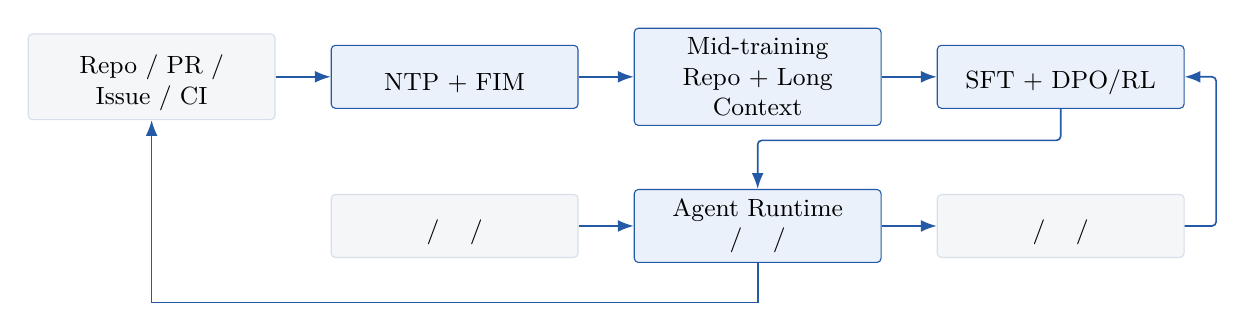
\begin{tikzpicture}[
  node distance=5mm and 7mm,
  box/.style={draw=LinkBlue,fill=PaleBlue,rounded corners=1.5pt,minimum height=8mm,text width=29mm,align=center,font=\small},
  data/.style={draw=CoolGray,fill=CodeBg,rounded corners=1.5pt,minimum height=8mm,text width=29mm,align=center,font=\small},
  arr/.style={-{Latex[length=2mm]},draw=LinkBlue,line width=.6pt}
]
\node[data] (raw) {代码与开发历史\\Repo / PR / Issue / CI};
\node[box,right=of raw] (pre) {预训练\\NTP + FIM};
\node[box,right=of pre] (mid) {Mid-training\\Repo + Long Context};
\node[box,right=of mid] (post) {后训练\\SFT + DPO/RL};
\node[box,below=8mm of mid] (agent) {Agent Runtime\\检索 / 编辑 / 执行};
\node[data,left=of agent] (env) {可执行环境\\版本 / 依赖 / 测试};
\node[data,right=of agent] (eval) {分层评估\\能力 / 成本 / 风险};
\draw[arr] (raw.east) -- (pre.west);
\draw[arr] (pre.east) -- (mid.west);
\draw[arr] (mid.east) -- (post.west);
\draw[arr,rounded corners=1.5pt] (post.south) -- ++(0,-4mm) -| (agent.north);
\draw[arr] (env.east) -- (agent.west);
\draw[arr] (agent.east) -- (eval.west);
\draw[arr,rounded corners=1.5pt] (eval.east) -- ++(4mm,0) |- (post.east);
\draw[arr] (agent.south) -- ++(0,-5mm) -| (raw.south);
\end{tikzpicture}
\caption{Code Agent 的四线闭环。训练数据必须保留到可执行环境与评估结果的血缘，运行轨迹再回流为下一轮 SFT、偏好或 verifier 数据。}
\label{fig:architecture}
\end{figure}

\Cref{fig:architecture}中的关键不是阶段顺序，而是四条线同步推进：模型训练没有执行环境就无法获得可靠奖励；环境没有数据血缘就无法去污染；评估没有固定 scaffold 和预算就无法区分模型收益；轨迹回流没有失败类型和版本信息就会把偶然成功当成可迁移策略。

\begin{table}[htbp]
\centering
\caption{各阶段应形成的独立验收面}
\label{tab:surfaces}
\small
\begin{tabularx}{\textwidth}{p{2.6cm}YYY}
\toprule
阶段 & 训练目标 & 主要数据 & 不可替代的验收 \\
\midrule
预训练 & 代码分布、局部补全、语义与修改先验 & source code、文档、Notebook、Issue/PR/Commit & HumanEval/MBPP 等、FIM、语言分项、held-out loss \\
Mid-training & 跨文件依赖、仓库结构、长距离定位与编辑 & repo pack、依赖图、PR diff、长 code-related 文本 & CrossCodeEval、RepoBench、长度分桶、跨文件检索/补全 \\
后训练 & 指令遵循、工具协议、决策与自修复 & 多轮轨迹、偏好对、可执行任务、失败反馈 & tool-call validity、loop rate、patch apply、resolve rate \\
Runtime & 安全地把策略映射为真实动作 & ACI、沙箱、索引、测试、缓存 & latency、成本、越权率、人工接管率、可审计性 \\
持续评估 & 新鲜度与部署分布鲁棒性 & live tasks、私有回归集、线上回放 & 去污染、同预算、同 scaffold、时间切片、版本可复现 \\
\bottomrule
\end{tabularx}
\end{table}

\section{预训练：先建立高质量代码与修改先验}

\subsection{数据组成不是“纯代码越多越好”}

公开技术报告已给出两类互补证据。OpenCoder 的 RefineCode 包含源代码与 code-related Web 数据，并强调 exact + file-level fuzzy dedup、语言特定过滤和 code-related recall\cite{huang2024opencoder}；Qwen2.5-Coder 报告的消融中，70\% Code、20\% Text、10\% Math 的组合优于纯代码设置，但这是特定模型与数据规模下的报告结果，不能直接外推为通用最优配比\cite{hui2024qwen25coder}。StarCoder2/The Stack v2 则提供了更透明的许可证检测、Software Heritage 血缘以及 Issue、PR、Notebook、文档等多源组成\cite{lozhkov2024starcoder2}。

建议把预训练池划分为以下互斥或可追踪的逻辑域：

\begin{itemize}
  \item \textbf{Source Code}：主干快照、历史版本、测试、配置、构建脚本、IDL 与数据库 schema；
  \item \textbf{Code-related Text}：官方文档、教程、README、设计文档、API reference、技术问答；
  \item \textbf{Development History}：Commit message/diff、PR 讨论、Issue、review comment、CI 日志；
  \item \textbf{Executable/Synthetic}：可编译样本、带单测的合成题、执行过滤后的 text-to-code；
  \item \textbf{General/Math}：维持指令理解、推理和非代码知识的受控通用数据。
\end{itemize}

不要让多个域在物理层重复计 token。例如 PR diff 中的 before/after 文件若又以快照形式进入 source code，需要建立 content hash 与 commit lineage，至少能报告 unique token、repeated token 和 actual trained token。

\subsection{清洗、过滤与去重}

代码数据质量需同时处理“文件是否像代码”“代码是否有学习价值”“数据是否重复”“许可证/隐私是否允许使用”四个问题。推荐 pipeline 为：格式识别 $\rightarrow$ exact dedup $\rightarrow$ 基础清洗 $\rightarrow$ 语言特定解析 $\rightarrow$ 质量/价值过滤 $\rightarrow$ fuzzy dedup $\rightarrow$ 污染剔除 $\rightarrow$ 配比采样。把 exact dedup 提前可以显著降低后续计算量；OpenCoder 报告其原始池中存在大量完全重复文件，并在自身消融中发现 file-level fuzzy dedup 优于 repo-level dedup\cite{huang2024opencoder}。这一结论说明“repo 作为组织单元”和“repo 作为去重单元”不应混淆：保留仓库结构并不要求以整个仓库做相似度判定。

对每个语言族，应分别维护：解析成功率、generated/vendor/test/config 识别率、规则触发率、人工误杀率、保留 token、去重 ratio 和 benchmark contamination hit。对代码专项尤其要避免以下误伤：高密度符号的 C/C++ 宏、短但关键的接口/类型声明、模板生成代码、测试 fixture、SQL/配置以及跨语言 binding。

定义第 $d$ 个数据域的采样权重 $w_d$、样本质量 $q_i$ 和温度 $T$，可采用受约束加权采样：

\begin{equation}
p(i)=\frac{w_{d(i)}\exp(q_i/T)}{\sum_j w_{d(j)}\exp(q_j/T)},
\qquad
\mathcal{L}_{\mathrm{pre}}=-\sum_i p(i)\sum_t m_{i,t}\log p_\theta(x_{i,t}\mid x_{i,<t}),
\label{eq:pretrain}
\end{equation}

其中 $m_{i,t}$ 允许屏蔽许可证声明、模板边界或仅对 FIM middle 计损失。$T$ 过低会使高分模板过度集中并损失多样性；$w_d$ 需要用等 token 小模型消融确定，而非由原始数据量决定。

\subsection{训练目标：NTP、FIM 与修改建模}

Next-token prediction（NTP）仍是基础，但 Code Agent 需要额外学习“在已有上下文中插入和修改”。FIM 将原序列拆为 prefix、middle、suffix，并以

\begin{equation}
\tilde{x}=[\mathrm{PRE};x_{<l};\mathrm{SUF};x_{>r};\mathrm{MID};x_{l:r}]
\label{eq:fim}
\end{equation}

进行自回归训练。DeepSeek-Coder 在 project-level code 上使用 FIM 并把训练窗口扩到 16K\cite{guo2024deepseekcoder}；Qwen2.5-Coder 则先做 8K file-level NTP/FIM，再做 32K repo-level FIM，并通过 YaRN 支持更长推理窗口\cite{hui2024qwen25coder}。工程上应联合消融 FIM rate、PSM/SPM 格式、middle 长度、跨文件目标位置和 loss mask，避免只在 HumanEval-FIM 上调参。

开发历史提供第三类监督：$\text{intent} + \text{before} \rightarrow \text{after/diff}$。OctoPack 将 Git commit 组织为自然指令与修改对，说明 commit 可作为跨语言修复/解释信号\cite{muennighoff2023octopack}；Clean-PR 进一步以经过严格过滤的真实 PR 做 repo-level mid-training，并强调 patch 可应用性与去污染\cite{lo2026cleanpr}。建议预训练只引入高置信的局部修改序列，复杂 PR 留到 mid-training，以减少输入噪声和目标歧义。

\section{数据收集：代码、PR/Issue 与轨迹必须共享血缘}

\subsection{统一数据对象}

一个可持续的数据平台不应维护相互割裂的“预训练 JSONL”“SFT 对话”和“评估实例”。建议以 \ident{repository snapshot} 为根对象，向下连接文件、符号、Issue、PR、Commit、环境、任务、轨迹和评估结果。最小 lineage 至少包含：repo URL、license、base commit、target commit、file hashes、采集时间、数据 split、构建镜像 digest、测试命令、模型/scaffold 版本和污染标签。

\begin{lstlisting}[style=codeblock,caption={建议的统一任务与轨迹记录（示意）},label={lst:schema}]
{
  "task_id": "repo@base_commit#issue_or_synthetic_id",
  "repo": {"url": "...", "base_commit": "...", "license": "..."},
  "problem": {"text": "...", "source": "issue|pr|synthetic"},
  "environment": {"image_digest": "sha256:...", "test_cmd": "..."},
  "oracle": {"patch_hash": "...", "fail_to_pass": [], "pass_to_pass": []},
  "trajectory": [{"observation": "...", "action": "...", "result": "..."}],
  "outcome": {"resolved": false, "failure_type": "localization"},
  "provenance": {"collected_at": "...", "split": "train", "contamination": []}
}
\end{lstlisting}

\subsection{真实任务、合成任务与轨迹数据}

真实 Issue/PR 的优势是意图、讨论和修改都来自开发过程，但存在关联错误、环境腐化、隐藏依赖、合并噪声与测试不足。合成任务更容易规模化并控制难度，但可能学习到生成器特征。SWE-Gym 提供 2,438 个带可执行环境的真实 Python 任务，并公开成功轨迹；其 rejection-sampling SFT 显示少量高质量多轮轨迹就能显著减少循环与空 patch\cite{pan2024swegym}。SWE-smith 先为仓库建立共享环境，再用函数重写、程序化 mutation、组合 bug 和 PR mirror 合成任务，报告 128 个仓库上约 50K 实例，并用 5,016 条专家轨迹训练模型\cite{yang2025swesmith}。R2E-Gym 使用测试生成和 commit back-translation 构造 8.7K 级环境，并研究执行式/非执行式 verifier 的互补性\cite{jain2025r2egym}。SWE-rebench 则面向持续采集和新鲜评估，公开超过 21K 个 Python 交互任务，并显式讨论污染\cite{badertdinov2025swerebench}。

由这些工作可归纳出四条工程规则：

\begin{enumerate}
  \item \textbf{Environment first}：先证明 base commit 可安装且基线测试稳定，再生成或接入任务；
  \item \textbf{双重验证}：gold patch 应实现 F2P，同时保持 P2P；重复运行以剔除 flaky test；
  \item \textbf{成功与失败并收}：成功轨迹用于行为克隆，失败轨迹用于 preference、verifier、failure classifier 和 curriculum；
  \item \textbf{按实例限额}：同一易题的大量成功采样会造成 easy-task bias，应按 task/repo cap 并报告去重后轨迹数。
\end{enumerate}

\subsection{轨迹质量与失败标签}

轨迹应分解为可诊断阶段，而非只有最终 reward：问题理解、文件定位、符号定位、错误复现、方案生成、patch apply、局部测试、回归测试、终止判断。建议保留以下失败标签：\ident{env\_setup}、\ident{localization}、\ident{reasoning}、\ident{edit\_syntax}、\ident{test\_generation}、\ident{regression}、\ident{loop}、\ident{budget}、\ident{unsafe\_action}、\ident{invalid\_task}。标签可由规则、执行信号和 LLM judge 联合产生，但 judge 只能做软标签，不能替代测试事实。

轨迹价值不应只按成功筛选。可定义：

\begin{equation}
v(\tau)=\alpha r_{\mathrm{exec}}+\beta r_{\mathrm{progress}}+\gamma d_{\mathrm{novelty}}-\delta c_{\mathrm{tokens}}-\eta r_{\mathrm{risk}},
\label{eq:trajectory-value}
\end{equation}

其中 $r_{\mathrm{progress}}$ 可由定位正确、复现成功、减少失败测试数等 dense signals 构成；$d_{\mathrm{novelty}}$ 用 task/repo/action n-gram 或 embedding 多样性近似。式\eqref{eq:trajectory-value}是工程建议，并非公开论文的统一定义。

\section{Mid-training：从单文件模型迁移到仓库级编辑}

\subsection{Repo-level 组织的三个层次}

仓库数据组织至少有三种粒度：

\begin{enumerate}
  \item \textbf{同仓随机拼接}：保留 repo 边界和 file path，但不显式编码依赖；成本最低，是必要 baseline；
  \item \textbf{结构感知拼接}：按 import、call、inherit、test-to-source、build dependency 排序或采样；
  \item \textbf{任务条件组织}：围绕 target symbol/issue 构建局部子图，加入 hard negative 与 oracle context。
\end{enumerate}

DeepSeek-Coder 与 StarCoder2 证明了 project/repository-level 序列可用于开放代码模型训练\cite{guo2024deepseekcoder,lozhkov2024starcoder2}；但“把同一 repo 文件塞入同一窗口”不自动证明模型学会了依赖关系。CrossCodeEval 明确要求跨文件上下文，并覆盖 Python、Java、TypeScript 和 C\#\cite{ding2023crosscodeeval}；RepoBench 则把 retrieval、completion 和 pipeline 拆分评估\cite{liu2023repobench}。因此，多层引用（DFS/BFS）、file-level、same-repo shuffled 和 dependency-aware 必须在等 token、等语言配比、等上下文长度下比较。

推荐的 8K/32K pack 由以下单元组成：目标文件局部上下文 + 直接依赖 + 测试/调用方 + 文档/Issue + 难负例。若窗口不足，优先保留声明、签名、类型、调用点和测试，而非完整实现。线上 runtime 的检索策略应与 mid-training 的上下文分布一致，否则训练时依赖 oracle context、推理时依赖低 recall 检索会产生明显分布偏移。

\subsection{PR/Issue 作为 mid-training 信号}

PR/Issue 数据连接“用户意图--仓库状态--修改--讨论--测试”，是从代码模型向编辑模型迁移的天然桥梁。建议形成多任务：

\begin{itemize}
  \item Issue $\rightarrow$ changed files / symbols（定位）；
  \item Issue + local tree $\rightarrow$ inspection actions（检索策略）；
  \item before + intent $\rightarrow$ diff / \ident{str\_replace}（修改）；
  \item diff + source $\rightarrow$ tests（单测生成）；
  \item candidate patch + logs $\rightarrow$ critique / repair（自修复）；
  \item PR discussion $\rightarrow$ review decision / revised patch（代码审查）。
\end{itemize}

Clean-PR 的最新公开结果支持把经过严格筛选、patch 可应用且去污染的 PR 用作 mid-training 信号，但其具体收益依赖所用模型、过滤器和评估 scaffold\cite{lo2026cleanpr}。工程上应先测 \metric{file recall@k}、\metric{symbol recall@k}、patch apply rate、edit exactness 和 held-out trajectory loss，再看端到端 resolve；这样能区分“学会定位”“学会编辑”和“scaffold 补救”。

\section{长上下文扩展：目标是有效利用，不是配置值变大}

\subsection{位置扩展、数据适配与系统成本}

RoPE 将第 $m$ 个位置映射为按维度旋转的表示。对第 $i$ 个二维通道，其相位可写为

\begin{equation}
\phi_i(m)=m\theta_i,\qquad \theta_i=b^{-2i/d}.
\label{eq:rope}
\end{equation}

超出训练长度时，$\phi_i(m)$ 进入 OOD 区域。YaRN 通过频率分区、插值与 attention scaling 降低扩窗训练成本\cite{peng2023yarn}；LongRoPE 进一步搜索非均匀插值并采用渐进式扩展\cite{ding2024longrope}。这些方法解决的是位置表示与训练稳定性，不保证模型具备仓库级多跳推理。LongAlign 的结论也指出，长上下文模型需要相近长度的指令数据，并需处理 packing 与 loss weighting\cite{bai2024longalign}。

标准全注意力的计算和激活随长度近似为

\begin{equation}
C_{\mathrm{attn}}=\mathcal{O}(L^2 d),\qquad M_{\mathrm{KV}}=\mathcal{O}(L\,n_{\mathrm{layer}}\,d_{\mathrm{kv}}),
\label{eq:long-cost}
\end{equation}

因此从 32K 扩到 128K 不是单纯改 \ident{rope\_theta}：需要 sequence parallel/context parallel、FlashAttention、长度分桶、packing、checkpointing、KV cache 策略与推理预算共同设计。Code Agent 还应问：是否真的需要把整个 repo 放进窗口，还是用 32K--64K 高 recall 检索 + 迭代查看更划算。

\subsection{建议的长上下文课程}

\begin{table}[htbp]
\centering
\caption{长上下文训练课程与门禁}
\label{tab:long-curriculum}
\small
\begin{tabularx}{\textwidth}{p{2.2cm}p{2.5cm}YY}
\toprule
阶段 & 长度分布 & 数据组织 & 门禁 \\
\midrule
L0 保能力 & 4K--8K 为主 & file-level NTP/FIM + 通用/数学 replay & 短上下文 benchmark 不显著回退 \\
L1 位置适配 & 8K/16K/32K 混合 & same-repo pack + 长文档 & 长度分桶 PPL、passkey、多 needle \\
L2 结构学习 & 16K--64K & dependency-aware、多层引用、target-aware & CrossCodeEval/RepoBench 随有效 context 提升 \\
L3 指令对齐 & 32K--128K 少量 & 长 Issue、目录、轨迹、multi-file diff & 长程定位、计划保持、工具协议不退化 \\
L4 推理优化 & 真实分布 & 检索压缩、KV/reuse、迭代浏览 & 同成功率下降低 latency/token cost \\
\bottomrule
\end{tabularx}
\end{table}

训练 mixture 不能只用最大长度。建议每个 batch bucket 明确 token 占比，保留 30\%--60\% 短序列 replay 作为初始探索范围，并以实验调节。RULER 表明 vanilla needle 准确率可能掩盖 multi-hop 和 aggregation 退化\cite{hsieh2024ruler}，所以长代码评估还必须加入跨文件引用链深度、干扰文件数量、target 位置和 repo size 分桶。

\section{后训练：从“会回答”到“会行动并验证”}

\subsection{SFT：先学稳定协议与基本策略}

SFT 数据至少覆盖三类：原子工具技能、结构化工作流和自由多轮轨迹。原子技能包括 search/view/edit/test/git diff；结构化工作流包括定位--修改--验证；自由轨迹覆盖根据执行反馈动态修正。CodeAct 用可执行 Python 统一动作空间，并公开 7K 多轮交互数据，说明“动作表示”本身会影响 Agent 学习\cite{wang2024codeact}。SWE-agent 强调 ACI 对导航、编辑和测试行为的影响\cite{yang2024sweagent}。

训练 mask 应区分 system/tool schema、observation、reasoning 和 action。若产品不输出显式思维链，可将可审计的短计划、状态摘要和动作理由作为训练目标，而不依赖长篇自由推理。SFT 关键指标包括 tool-call parse rate、action validity、empty patch、loop rate、平均 turns、无效读取比例和 test-before-finish 比率。

\subsection{偏好优化与 verifier}

偏好对可由同题多轨迹构造：成功优于失败；无回归优于只过新增测试；更小且解释充分的 patch 优于大范围改写；相同成功下低成本优于高成本。DPO 可在不在线采样的情况下学习相对偏好，但若 preference 主要由 judge 产生，模型会学习 judge 风格和长度偏差。应混合执行事实、人工 rubric 与模型评分，并单独评估 reward hacking。

Outcome verifier 对轨迹 $\tau$ 和 patch $P$ 估计

\begin{equation}
s_{\phi}(\tau,P)=P_{\phi}(\mathrm{YES}\mid \text{task},\tau,P),
\label{eq:verifier}
\end{equation}

用于 Best@$k$ 选择或过程 pruning。SWE-Gym 使用成功/失败轨迹训练 outcome-supervised verifier\cite{pan2024swegym}；R2E-Gym 发现 execution-based 与 execution-free verifier 各有盲区，组合后更有效\cite{jain2025r2egym}。因此 production verifier 应由回归测试、定向测试生成、静态分析、diff risk 与 learned score 共同组成，而不是单一 reward model。

\subsection{为什么 Code Agent RL 不是普通的单轮 RLVR}

RL 是 Code Agent 从“模仿成功轨迹”走向“依据环境反馈主动探索”的关键模块，但软件工程任务同时具有\textbf{状态可变、轨迹极长、奖励稀疏、环境昂贵且会失败}四个特征。数学/竞赛代码 RLVR 通常只需对一个完整输出判分；Code Agent 则要在几十轮工具交互和数万至十余万 token 后，才由隐藏测试给出终局奖励。Long-Context Multi-Turn SWE RL 的公开实验把这种差异形式化为 stateful MDP，并指出把一个 terminal advantage 广播给整条轨迹会产生严重信用分配噪声\cite{golubev2025longcontextrl}。

因此，训练前应满足三个先决条件：其一，SFT/RFT 初始策略在训练题上已有非零 pass@$k$，否则同组 rollout 全为零，group-relative advantage 不可用；其二，gold patch、空 patch 和重复运行能验证 evaluator 的确定性；其三，容器启动、依赖安装、测试 flaky 等基础设施失败能够与 policy failure 分离。RL 提升的直接对象不是“代码知识总量”，而是\emph{搜索顺序、试验选择、失败恢复、终止与提交}这些闭环策略。

\subsection{四条已被实践验证的技术路线}

\subsubsection{路线 A：基于软件演化数据的 proxy-reward RL}

SWE-RL 从 GitHub Issue/PR 构造 issue、pre-change context 与 oracle patch，使用预测 patch 和 oracle patch 的序列相似度作为连续 reward，并以 GRPO 优化\cite{wei2025swerl}。这种方法不需要启动完整仓库环境，吞吐高、易扩展，连续相似度也比“是否完全匹配”的离散 reward 更密集。其局限同样明确：patch 文本相似不等价于语义正确，会惩罚与开发者实现不同但有效的 patch；且其主训练任务给定相关代码上下文，弱化了真实 Agent 的定位与多轮执行难度。它更适合做大规模 reasoning/editing warm-up，而不应作为最终 agentic reward。

\subsubsection{路线 B：真实执行环境中的长轨迹 RL}

执行型 RL 直接以 F2P/P2P 测试判定 patch。Golubev 等人在 131K context 的多轮环境中采用 RFT 冷启动和修改后的 DAPO：每题采样 10 条完整轨迹、组内归一化 terminal reward、丢弃零 advantage 组，并加入轨迹长度惩罚；在相同 scaffold 下从 20\% 的 RFT baseline 提升到 39\% SWE-bench Verified\cite{golubev2025longcontextrl}。论文也警告：事后截断超窗轨迹会造成 rollout policy 与训练 log-prob 不一致，破坏 importance sampling 假设。

SWE-Master 给出了更工程化的稳定策略\cite{song2026swemaster}：先对约 60K 条长轨迹 SFT，再在 Docker 环境中做 GRPO；以 leave-one-out advantage、固定长度归一化、clip-higher 和去 KL 维持探索；对预算耗尽轨迹强制提交当前 patch，并按 stop reason 折扣 reward；容器/服务失败直接 mask，不进入 policy update；每轮 observation 显式返回剩余预算。其重要启发不是某个单独超参，而是\textbf{termination semantics 和 infrastructure semantics 必须进入 RL 数据模型}。

\subsubsection{路线 C：用 guidance 或子能力分解降低稀疏性}

Agent-RLVR 让 Agent 先自行尝试，对失败轨迹再提供 plan、错误纠正或环境交互提示，重新 rollout 后用可验证 reward 更新；guidance 只在训练采样时出现，推理时移除\cite{da2025agentrlvr}。其 Qwen2.5-72B-Instruct 在 SWE-bench Verified 上由 9.4\% 提升到 22.4\%，再用同批轨迹训练 reward model 做候选排序达到 27.8\%。这说明 teacher 的价值可以是\emph{让稀疏奖励区域出现成功样本}，而不一定把完整答案蒸馏给学生；但需要检查模型是否依赖 guidance 风格，以及 teacher 是否泄露 gold 信息。

另一种做法是先训练可密集判分的原子策略。CodeScout 把 code localization 定义为 file/module/function 三粒度集合预测，使用三者 F1 之和作为 reward，Agent 仅用 Unix terminal 搜索并通过结构化 finish tool 提交\cite{sutawika2026codescout}。这一设计把 reward 从“最终 patch 是否完全正确”变为“相关位置找得多准”，同时避免脆弱字符串解析。子能力 RL 应与端到端 RL 串联验证：定位 F1 上升只有在固定 repair model、固定 budget 下提升 resolve rate，才算形成有效迁移。

\subsubsection{路线 D：自博弈生成难度递增的可执行课程}

Self-play SWE-RL 让同一 policy 交替扮演 bug injector 和 solver：注入端从真实仓库生成 bug patch 与 test-weakening patch，通过一致性检查过滤不可执行样本；solver 在隐藏测试约束下修复；注入 reward 鼓励“有效、非平凡、但仍可解”的 bug，而不是越难越好\cite{wei2025selfplay}。该方法在不依赖人类 Issue/PR 标注的设置中报告 SWE-bench Verified 和 SWE-Bench Pro 分别提升 10.4 与 7.8 个点。其关键风险是自博弈分布退化：注入器可能学习人工化、易判分却不符合真实缺陷的模式，因此必须监控 bug type、修改范围、语言/repo 分布及对真实 Issue 的迁移。

\begin{table}[htbp]
\centering
\caption{Code Agent RL 路线的信号、优势与主要偏差}
\label{tab:rl-routes}
\small
\begin{tabularx}{\textwidth}{p{2.2cm}p{3.2cm}YY}
\toprule
路线 & 主要 reward & 适合解决的问题 & 主要偏差/门禁 \\
\midrule
Proxy patch RL & oracle patch 相似度、格式 & 低成本 reasoning/editing warm-up & 等价 patch 误罚；必须用执行评测复核 \\
Execution RL & F2P/P2P、回归与终止折扣 & 端到端搜索--编辑--验证策略 & 环境吞吐、flaky、稀疏奖励与长程信用 \\
Guided / skill RL & guided success、定位 F1、过程里程碑 & 冷启动、定位/测试等瓶颈能力 & guidance 泄露、proxy 与 resolve rate 脱钩 \\
Self-play RL & bug 有效性、目标难度、修复成功 & 扩展任务分布和自动课程 & 合成缺陷模式坍缩；需真实任务迁移门禁 \\
\bottomrule
\end{tabularx}
\end{table}

\subsection{奖励、优化与信用分配的可落地配方}

执行 reward 不应只保留一个 success bit。建议保留可审计的向量，再在训练侧组合：

\begin{equation}
\begin{aligned}
r(\tau)=&\ \alpha r_{\mathrm{F2P}}+\beta r_{\mathrm{P2P}}+\gamma r_{\mathrm{progress}}
+\eta r_{\mathrm{submit}} \\
&-\lambda_1 c_{\mathrm{turn}}-\lambda_2 r_{\mathrm{unsafe}}
-\lambda_3 r_{\mathrm{test\,tamper}}-\lambda_4 r_{\mathrm{scope}} .
\end{aligned}
\label{eq:reward}
\end{equation}

$r_{\mathrm{progress}}$ 只能来自较难投机的证据，如编译错误减少、目标测试通过子集增加、复现测试从 pass 变 fail、静态类型错误收敛；不能直接奖励“调用了测试”“读取了文件”等表面动作。$r_{\mathrm{submit}}$ 区分主动提交和预算耗尽后的强制提交；$r_{\mathrm{scope}}$ 约束无关文件和 diff 扩张。删除/放宽测试、硬编码样例、修改 grader、绕过依赖、写环境外部状态都应由独立 rule-based detector 触发 hard zero 或样本剔除。

优化上可采用 GRPO/GSPO/DAPO 类无 critic 方法作为起点，但要记录 group success diversity：若同组全成功或全失败，更新信号为零；若高难题长期全零，应提高 rollout 数、加入 guidance/课程或回退到 rejection fine-tuning，而不是盲目拉长训练。对超长轨迹，单一 trajectory advantage 广播到所有 token 只是基线。进一步方案包括：（1）从共享 prefix 分叉 rollout，比较后续动作的反事实价值；（2）用可验证 milestone 产生 step/segment reward；（3）训练 critic/value head 做局部 advantage；（4）只对模型 action token 求 loss，mask tool observation 和基础设施异常。过程 reward 越密，越要检查是否诱导“刷进度”而非完成任务。

\subsection{RL 系统、数据血缘与实验归因}

训练系统至少包含 environment pool、rollout workers、trajectory/event store、reward/evaluator、trainer 和 checkpoint broadcaster。每条样本必须绑定 repo commit、container digest、test patch、harness/scaffold commit、model revision、sampling seed、stop reason、reward components 与 artifact URI。异步 rollout 能提高 GPU/CPU 利用率，但旧 checkpoint 产生的 trajectory 会增加 off-policy staleness；应记录 policy version 并设置最大滞后，而不是把所有轨迹混为同一分布。

最小因果实验矩阵应固定 base/SFT checkpoint、task split、harness、context、turn/token budget 和 rollout 总数，比较：SFT/RFT、offline preference、proxy-reward RL、execution RL、execution RL + guidance、execution RL + process signal，以及不更新参数的 best-of-$k$ + verifier。主指标除 resolve rate 外，还应报告 pass@$k$、group nonzero rate、reward/entropy、active-submit rate、forced-submit success、environment mask rate、平均 turns/tokens、diff size、回归/越权率和 unseen-repo 迁移。只有在\textbf{相同采样预算}下胜过 SFT 与 test-time scaling，且在 held-out repo 上保持收益，才能把提升归因于 policy learning。

\section{Agent Runtime：让模型在受控接口中工作}

\subsection{最小而充分的工具面}

基础工具建议限制为：目录/符号搜索、文件分段读取、结构化编辑、终端执行、测试、diff/status 与最终提交。工具应返回稳定、可解析且长度受控的 observation；编辑工具必须验证 old text 唯一匹配或基于 patch apply；终端需限制网络、文件系统和进程权限。OpenHands 将终端、编辑器与浏览器等置于沙箱平台\cite{wang2024openhands}，但在企业代码场景还需增加 secret redaction、依赖源 allowlist、审计日志和人工审批门。

运行时不应默认“全 repo 注入”。更稳健的上下文管理包括：repo map、symbol graph、BM25/embedding 混合检索、最近 observation 压缩、persistent scratchpad 与 diff-aware cache。Agent 每轮应得到当前目标、已知事实、工作区状态和剩余预算，而不是不断拼接原始历史。

\subsection{Harness：连接模型策略与可执行世界的控制平面}

\textbf{Harness 不等于 scaffold，也不等于 evaluation harness。} Scaffold 定义模型看到的 prompt、工具与行动风格；agent harness 负责把一次任务可靠地运行成完整 episode；environment 提供仓库与执行隔离；evaluation harness 则在 episode 结束后应用 patch、运行标准测试并判分。一个结果应明确写成

\begin{equation}
Y=f(M,S,H,E,V,B,\xi),
\label{eq:harness-factorization}
\end{equation}

其中 $M$ 为模型 checkpoint，$S$ 为 scaffold/prompt，$H$ 为 agent harness，$E$ 为环境镜像，$V$ 为 evaluator/verifier，$B$ 为预算，$\xi$ 为采样随机性。只报告“模型名 + SWE-bench 分数”无法复现式\eqref{eq:harness-factorization}中的其余变量。

Agent harness 应实现一个显式 episode 状态机：\ident{INIT} $\rightarrow$ \ident{OBSERVE} $\rightarrow$ \ident{MODEL\_STEP} $\rightarrow$ \ident{PARSE/POLICY} $\rightarrow$ \ident{EXECUTE} $\rightarrow$ \ident{UPDATE}，在成功、失败、超时、预算耗尽、越权或人工中断时进入终态。每个转移都要幂等或可判定是否已执行，避免模型/API 重试造成同一写操作重复发生。

\begin{table}[htbp]
\centering
\caption{Code Agent harness 的核心模块与验收点}
\label{tab:harness}
\small
\begin{tabularx}{\textwidth}{p{2.8cm}YY}
\toprule
模块 & 职责 & 必测故障与指标 \\
\midrule
Episode Orchestrator & 状态机、终止条件、重试、checkpoint/resume & 重复执行、死循环、恢复一致性、terminal reason 分布 \\
Model Adapter & 统一 chat/response/tool-call、流式输出与 token accounting & schema 差异、截断、rate limit、实际输入/输出 token \\
Context Manager & history、repo map、检索、压缩、cache 与 context budget & 信息丢失、超窗、cache stale、有效 context 命中率 \\
Action Parser/Policy & 解析动作、参数校验、allow/deny/approval、去重 & parse rate、invalid action、越权阻断、审批次数 \\
Environment Adapter & local/container/remote sandbox、workspace 与进程生命周期 & base commit 漂移、僵尸进程、网络/文件越界、资源泄漏 \\
Tool Runtime & search/view/edit/shell/test/git 的超时、输出截断和错误映射 & command timeout、partial output、patch 冲突、工具错误率 \\
Budget Controller & turns、tokens、wall time、cost、CPU/GPU/IO 限额 & 超预算动作、预算估计偏差、成功成本分布 \\
Event Store & append-only event、artifact、diff、日志、trace 与 replay & 丢事件、敏感信息、trace 可重放率、版本字段完整率 \\
Evaluator Bridge & 生成标准 prediction、提交 evaluation harness、收集细粒度结果 & patch serialization、F2P/P2P、gold sanity、评测超时 \\
\bottomrule
\end{tabularx}
\end{table}

Harness 的设计复杂度应与研究问题匹配。SWE-agent 适合研究工具集合、history processor 和 ACI；mini-SWE-agent 则用线性消息历史、独立 shell action 和极小控制流，把研究焦点放回模型本身\cite{minisweagent2026}。两者没有绝对优劣：复杂 harness 便于加入 guardrail、检索与恢复，最小 harness 更适合作为模型能力 baseline，并降低 scaffold overfitting。

评估侧必须与 agent harness 解耦。SWE-bench 官方 evaluation harness 采用分层 Docker image，执行 setup、patch application、test、grading 和 reporting，并提供 cache、timeout 与日志控制\cite{swebenchharness2026}。内部评估也应先用 gold patch 做 harness sanity check，再测空 patch/错误 patch 的负控；否则环境或 grader 故障会被误记为模型失败。每次 run 至少冻结以下 manifest：

\begin{lstlisting}[style=codeblock,caption={Harness run manifest 的最小复现信息},label={lst:harness-manifest}]
run_id, task_set_version, model_id, model_api_revision,
scaffold_commit, harness_commit, prompt_hash, tool_schema_hash,
environment_image_digest, evaluator_commit, retriever_index_digest,
context_limit, max_turns, max_tokens, timeout_s, sampling_seed,
network_policy, permission_policy, cache_policy
\end{lstlisting}

对训练数据生产，harness 还要支持 deterministic replay 和 counterfactual replay：前者在冻结 observation 时重放 model/actions，检查 parser 与状态机一致性；后者替换模型或某一步 action，比较后续分支。若 observation 含时间、网络或并发等非确定状态，应保存原始事件和外部 artifact，而不是假设命令可再次产生相同输出。

\subsubsection{Claude Code：从公开接口重建 Harness 架构剖面}

Claude Code 的完整内部实现并未公开，因此不能把产品行为反推成确定的私有模块图。可由官方文档和工程文章确认的，是一组\textbf{公开控制面}：模型在环境反馈驱动的 loop 中选择工具；Claude Agent SDK 暴露与 Claude Code 同源的工具、context management 和 permission primitives；项目指令、memory、compaction、subagent、hooks、MCP、permissions 与 sandbox 分别承担不同控制职责\cite{anthropic2024agents,anthropic2025bestpractices,anthropic2025autonomy}。据此可得到表\ref{tab:claude-code-public-architecture}，它是公开能力的工程映射，不是对闭源实现的逆向结论。

\begin{table}[htbp]
\centering
\caption{Claude Code 的公开 Harness 控制面及可迁移设计原则}
\label{tab:claude-code-public-architecture}
\small
\begin{tabularx}{\textwidth}{p{2.4cm}p{4.2cm}Y Y}
\toprule
控制面 & Claude Code 公开机制 & Harness 职责 & 对自建 Code Agent 的启发 \\
\midrule
上下文/记忆 & \ident{CLAUDE.md} 分层指令、auto memory、compaction & 注入项目规范，压缩历史，跨会话保留可复用事实 & 指令、工作记忆、长期记忆分库存储并记录 provenance\cite{claudecodememory2026} \\
工具/扩展 & Read/Edit/Bash、MCP、Skills & 统一 tool schema、observation 截断与外部连接 & 工具能力与权限分离；外部内容视为不可信输入 \\
确定性控制 & lifecycle hooks、settings、finish/stop 条件 & 格式化、审计、阻断保护文件、压缩后重注入 & 硬约束放 hook/policy，不依赖 prompt 自觉\cite{claudecodehooks2026} \\
任务隔离 & subagent 独立 context、tool/model/permission 配置 & 隔离高噪声检索/测试，返回结构化摘要 & delegation 必须记录输入摘要、agent 配置和 handoff artifact\cite{claudecodesubagents2026} \\
安全边界 & permission 先判工具；Bash 再受 OS sandbox 的文件/网络约束 & allow/ask/deny、最小权限、egress 与 workspace 隔离 & policy guard 与 OS enforcement 叠加，不能互相替代\cite{claudecodesandbox2026} \\
可恢复执行 & session resume、checkpoint、structured handoff & 跨 context/session 恢复状态与未完成任务 & 以文件/事件为真相源，恢复后先验证环境而非相信摘要 \\
\bottomrule
\end{tabularx}
\end{table}

长任务 Harness 的公开演进也很有启发。Anthropic 早期方案用 initializer agent 建立环境、任务清单和进度文件，再让 coding agent 每个 session 做增量工作并留下 handoff artifact，解决 context reset 后的失忆\cite{anthropic2025longharness}；后续应用构建方案扩展为 planner--generator--evaluator，生成器与评估器在每个 sprint 前协商可测试 contract，评估器用浏览器/执行反馈验收\cite{anthropic2026harnessdesign}。这两者是\emph{建立在 Claude Agent SDK 上的示例 Harness}，不应写成 Claude Code 默认内部拓扑。它们共同说明：长程自治的关键状态应落在 repo、任务表、测试契约和 event log 中，而不是只留在聊天上下文。

安全面同样体现双层控制。公开的 Claude Code sandbox 对 Bash 子进程使用 macOS Seatbelt 或 Linux bubblewrap 做 OS 级文件系统约束，并通过 sandbox 外代理实施域名 egress 控制；permission 则在工具运行前决定 allow/ask/deny，两者覆盖面不同\cite{claudecodesandbox2026}。Auto mode 的公开架构又增加输入侧 prompt-injection probe 和输出侧 tool-call classifier，subagent 递归经过相同管线\cite{anthropic2026automode}。对企业 Code Agent，等价实现至少应区分：\textbf{模型倾向约束、Harness policy、OS/容器强隔离、外部连接器权限}，并用攻击回放分别测每层是否真正生效。

\begin{keybox}[Harness 设计边界]
Harness 能显著抬高特定模型的任务成功率，但它编码了“模型当前做不到什么”的假设。模型升级后，应逐项移除 planner、强制阶段、额外 verifier 或 context reset 做消融；若分数不降，就删除该复杂度。反过来，任何声称模型能力提升的实验，都应先在 minimal harness 与 production harness 两个剖面复测，防止把 scaffold/harness overfitting 误记为 checkpoint 收益。
\end{keybox}

\subsection{自治程度与工作流选择}

不同应用应选择不同自治等级：

\begin{itemize}
  \item \textbf{L0 建议}：补全、解释、review comment，不能直接写仓库；
  \item \textbf{L1 受控编辑}：生成 patch，用户确认后执行；
  \item \textbf{L2 沙箱任务}：自主搜索、编辑和测试，但不能访问生产资源；
  \item \textbf{L3 工作流 Agent}：可建分支、提交 PR、响应 CI，关键动作审批；
  \item \textbf{L4 长程自治}：跨任务规划与持续运行，仅适合高可验证、强隔离场景。
\end{itemize}

Agentless 的结果说明，对于定位、修复、验证可明确分解的任务，固定 pipeline 可能更便宜且可解释\cite{xia2024agentless}。因此自治不是默认目标，而是当动态环境与分支决策确实带来收益时才逐级开放。

\section{评估体系：必须把模型、检索、scaffold 与预算解耦}

\subsection{四级评估矩阵}

\begin{longtable}{p{2.0cm}p{3.2cm}p{4.3cm}p{6.1cm}}
\caption{Code Agent 分层评估矩阵}\label{tab:eval-matrix}\\
\toprule
层级 & 代表任务/基准 & 核心指标 & 解释边界 \\
\midrule
\endfirsthead
\multicolumn{4}{l}{\small 表\thetable（续）}\\
\toprule
层级 & 代表任务/基准 & 核心指标 & 解释边界 \\
\midrule
\endhead
函数级 & HumanEval、MBPP、LiveCodeBench、BigCodeBench、DS-1000 & pass@1/pass@$k$、执行正确率、库调用覆盖 & 测语法、算法、指令和 API 使用；不能代表跨文件定位\cite{chen2021codex,jain2024livecodebench,zhuo2024bigcodebench,lai2022ds1000} \\
跨文件 & CrossCodeEval、RepoBench、FIM/repair suites & EM、Edit Similarity、CodeBLEU、retrieval recall@k & 应报告有/无 oracle context 与语言分项；不能直接代表多轮 Agent\cite{ding2023crosscodeeval,liu2023repobench} \\
仓库任务 & SWE-bench Verified/Multilingual、SWE-bench-Live、SWE-rebench & resolve rate、patch apply、F2P/P2P、成本 & 高度依赖环境、scaffold、预算与污染；必须固定版本\cite{jimenez2024swebench,badertdinov2025swerebench,microsoft2026swebenchlive} \\
产品闭环 & 私有 Issue、代码审查、迁移、测试生成、CI 修复 & 接受率、time-to-merge、revert、人工接管、风险、成本 & 最接近业务价值，但需对任务难度、用户与仓库分布做归一化 \\
\bottomrule
\end{longtable}

pass@$k$ 的无放回估计为\cite{chen2021codex}

\begin{equation}
\widehat{\mathrm{pass@}k}=1-\frac{\binom{n-c}{k}}{\binom{n}{k}},
\label{eq:passk}
\end{equation}

其中 $n$ 是采样数、$c$ 是正确样本数。对 Agent，应同时报告 pass@1、pass@$k$ 和 verifier-selected Best@$k$；三者对应单次策略、多样性上限和选择器能力，不能混写成同一分数。

\subsection{公平比较与污染控制}

端到端比较至少固定：base model checkpoint、context limit、prompt/scaffold、工具集合、检索器、最大 turns、token/美元预算、temperature、容器镜像、并发与重试。训练实验还必须固定总训练 token、语言配比、采样次数、序列长度分布与 optimizer steps。若 repo-level 方案训练了更多 epoch 或更多实际 token，loss/benchmark 上涨不能归因于组织策略。

污染治理建议四层并行：repo exclusion；文件/patch exact hash；代码 10--15 gram 或 MinHash 相似度；Issue/描述 embedding/Jaccard。时间切分以 Issue/PR 创建时间和模型 data cutoff 双重标记。LiveCodeBench 通过持续收集新竞赛题减轻静态代码基准污染\cite{jain2024livecodebench}；SWE-rebench 与 SWE-bench-Live 将“持续采集新鲜可执行任务”扩展到软件工程 Agent\cite{badertdinov2025swerebench,microsoft2026swebenchlive}。新鲜评估并不自动无污染，还需检查 repo 历史、派生 patch 和基础模型暴露。

\subsection{推荐 dashboard}

至少同时展示：

\begin{itemize}
  \item \textbf{能力}：resolve、F2P、P2P、file/symbol recall@k、tool-call validity；
  \item \textbf{效率}：tokens/task、turns/task、wall time、GPU/CPU/container hours、成功任务成本；
  \item \textbf{行为}：loop、empty patch、test execution、rollback、无效动作与 context utilization；
  \item \textbf{质量}：diff size、回归、静态告警、review 接受率、revert rate；
  \item \textbf{数据}：unique/actual token、dedup ratio、repo/language/task diversity、环境构建率；
  \item \textbf{风险}：secret exposure、越权、依赖供应链、测试篡改与 license violation。
\end{itemize}

\section{应用场景：按可验证性与风险选择落点}

\begin{table}[htbp]
\centering
\caption{应用场景、训练信号与上线门槛}
\label{tab:applications}
\small
\begin{tabularx}{\textwidth}{p{3.0cm}YYY}
\toprule
场景 & 关键能力/数据 & 主评估 & 建议自治级别 \\
\midrule
IDE 补全与编辑 & FIM、局部上下文、用户接受/撤销 & 接受率、edit survival、延迟 & L0--L1 \\
Repo 问答与定位 & repo map、符号图、Issue-to-files & recall@k、回答可引用性 & L0--L1 \\
Bug 修复/Issue-to-PR & PR/Issue、执行轨迹、回归测试 & resolve、P2P、人工接管 & L2--L3 \\
测试生成 & source-to-test、mutation、覆盖反馈 & mutation score、缺陷发现率 & L1--L2 \\
代码审查与安全修复 & PR discussion、静态扫描、CVE & precision/recall、误报、风险等级 & L0--L2 \\
重构/迁移 & 多文件 diff、build graph、API 版本 & build/test、语义等价、diff 风险 & L2--L3 \\
数据科学与分析自动化 & Notebook、DS-1000、库文档、执行 & execution、结果正确性、可复现 & L1--L2 \\
CI/DevOps 修复 & build log、workflow、依赖图 & pipeline recovery、供应链风险 & L2，关键动作审批 \\
\bottomrule
\end{tabularx}
\end{table}

优先落地应选择 reward 清晰、环境隔离、失败可回滚且人类审阅成本可控的场景。Issue-to-PR 很适合研究，但生产首站往往是定位、测试生成或受控 patch，因为它们更容易将模型收益与系统风险解耦。对安全修复、依赖升级和 CI，应把网络访问与发布权限放在独立执行器，不让语言模型直接持有长期凭据。

\section{实验路线图：用等 token 与分层指标建立因果证据}

\subsection{阶段 A：代码基座与数据 pipeline}

目标是证明数据质量与配比收益，而不是追求最大模型。建议先用 1B--3B proxy，固定 architecture、tokenizer、训练 token 和 batch token，比较：

\begin{enumerate}
  \item file exact + fuzzy dedup 的阈值与误杀率；
  \item code-only vs code+text vs code+text+math；
  \item rule filter、model filter、value filter 的独立和组合增益；
  \item code-related Web、Issue/PR/Commit 的增量价值；
  \item FIM rate 与多语言采样温度。
\end{enumerate}

门禁：每个候选同时给出 held-out loss trajectory、HumanEval/MBPP/LiveCodeBench、BigCodeBench、语言分项、unique token 和误杀抽检。训练效率应按达到同等 benchmark 的 token 数，而不只看最终分数。

\subsection{阶段 B：Repo-level 与长上下文}

核心 $2\times 2\times 2$ 消融为：file vs repo；same-repo shuffle vs dependency-aware；1-hop vs multi-hop。固定 8K 与 32K 实际训练 token，再增加 64K 小比例课程。报告：

\begin{itemize}
  \item file$\rightarrow$func 组织成功率、func$\rightarrow$file 还原一致率、遗漏 symbol/file 数；
  \item CrossCodeEval 四语言、RepoBench retrieval/completion/pipeline；
  \item target dependency depth、repo size、context length 和 target position 分桶；
  \item algorithm benchmark 安全线与短上下文回退；
  \item oracle context、训练同构 retriever 和真实 retriever 三种 setting。
\end{itemize}

如果 dependency-aware 只在 oracle context 下有效，应优先修检索；如果 same-repo shuffle 与 dependency-aware 接近，说明收益可能来自位置适配或同域长序列，而非图结构。

\subsection{阶段 C：轨迹学习与 Agent}

先固定一个最小 scaffold，在相同 32K context、turn budget 和 temperature 下比较：base、atomic-tool SFT、successful-trajectory SFT、success+failure preference、verifier Best@$k$、online RL。训练数据以 task/repo 去重后的轨迹数和 actual tokens 双报。建议关键消融包括：

\begin{itemize}
  \item 有/无 reasoning summary；有/无 execution observation；
  \item 真实 Issue vs PR mirror vs procedural/synthetic bugs；
  \item 单成功轨迹/题 vs 多轨迹/题；随机扩量 vs 新 repo/新任务扩量；
  \item outcome verifier vs process verifier vs execution verifier；
  \item 32B 单次采样 vs 较小模型 Best@$k$ 的等成本比较。
\end{itemize}

\begin{table}[htbp]
\centering
\caption{建议的阶段性 go/no-go 门槛（需按现有 baseline 校准）}
\label{tab:gates}
\small
\begin{tabularx}{\textwidth}{p{2.5cm}YYp{3.2cm}}
\toprule
阶段 & Go 条件 & No-go 信号 & 下一动作 \\
\midrule
数据 pipeline & 等 token 下多项代码评估稳定增益，误杀可解释 & 仅 loss 下降或只涨单一 benchmark & 做污染/重复审计与语言分桶 \\
Repo mid-train & 跨文件指标提升且算法安全线不退 & 只在更长输入或 oracle context 下提升 & 加 same-repo shuffle 与 retriever 控制 \\
长上下文 & 多 hop/aggregation 随长度保持，短任务不退 & 仅 passkey 成功，真实 repo 无增益 & 调整长数据与位置课程 \\
轨迹 SFT & resolve、loop、empty patch 同时改善 & 成功率涨但成本/回归恶化 & 加失败轨迹与成本/风险偏好 \\
RL/verifier & 等 rollout 成本优于 SFT/best-of-$k$ & reward 上升但私有集不涨 & 查 reward hacking 与环境噪声 \\
上线 & 私有任务接受率、回滚与风险达标 & benchmark 高但人工接管/成本过高 & 降自治级别、收窄场景 \\
\bottomrule
\end{tabularx}
\end{table}

\section{主要风险与开放问题}

\subsection{数据与法律边界}

公开可访问不等于可随意训练或再分发。应记录 repo/file 级许可证、删除请求、PII/secret 检测、生成代码归因与训练数据 provenance。The Stack v2 的 Software Heritage 标识与许可证流程提供了可审计范式\cite{lozhkov2024starcoder2}，但不同组织仍需结合使用地区和产品形态做法律评估。

\subsection{环境与测试不等于真实正确性}

测试可能不完整、脆弱或可被投机；旧仓库环境也可能因依赖消失而不可重现。任务构建率、基线稳定率、gold patch 验证率必须作为数据质量指标，而不是隐藏在 dataset size 后。SWE-smith、SWE-rebench 等工作都把环境构建视为主要成本与误差源\cite{yang2025swesmith,badertdinov2025swerebench}。

\subsection{基准饱和与系统共适应}

同一批仓库长期出现在训练、prompt 设计和 leaderboard 中，会导致模型、检索器和 scaffold 对基准共适应。应维护按月/季度滚动的 shadow set、私有任务和时间外推集，并冻结一套可复现 baseline。任何 SOTA 数字都应附带模型版本、scaffold commit、预算和日期。

\subsection{能力外推与安全}

从“能修 Python Issue”不能外推到多语言、大型 monorepo、分布式系统或生产发布。长程 Agent 还可能执行破坏性命令、泄露 secret 或引入供应链依赖。安全策略必须由沙箱、权限系统和 policy engine 强制执行，不能只依靠 prompt。

\section{总结与展望}

构建 Code Agent 的正确主线，是把代码模型训练与可执行软件工程环境统一起来。预训练解决“懂代码与修改模式”，mid-training 解决“理解仓库结构并利用长上下文”，后训练解决“按协议行动、从反馈修正”，runtime 解决“安全、低成本、可审计地执行”，持续评估则保证这些收益在新鲜任务上仍然成立。

短期最有确定性的投入不是盲目扩大模型或窗口，而是三项基础设施：第一，带许可证、commit、测试与 split 血缘的统一数据层；第二，可批量构建、缓存和复验的环境层；第三，固定 scaffold/预算、能拆分定位--编辑--验证的评估层。有了这三层，预训练数据策略、repo-level 组织、轨迹 SFT、verifier 与 RL 才能通过等 token、等成本实验获得可信归因。

中期的研究重点应从“更多成功轨迹”转向“覆盖更多 repo、语言、失败模式和依赖深度”，从“标称 128K”转向“在复杂干扰和多跳引用下的有效上下文”，从“单一 resolve rate”转向能力、成本、回归、安全和人工接管的联合 Pareto 前沿。长期看，Code Agent 的竞争力将更多来自数据与环境闭环，而非单次模型发布：系统能否把真实开发反馈快速转成干净、可执行、去污染的训练与评估实例，将决定迭代速度和可持续上限。

\clearpage
\appendix
\section{附录 A：数据与环境验收清单}

\begin{longtable}{p{3.0cm}p{5.8cm}p{7.3cm}}
\caption{生产数据 pipeline 的最小验收字段}\label{tab:data-checklist}\\
\toprule
对象 & 必备字段 & 核心指标/检查 \\
\midrule
\endfirsthead
\multicolumn{3}{l}{\small 表\thetable（续）}\\
\toprule
对象 & 必备字段 & 核心指标/检查 \\
\midrule
\endhead
Repository & URL、license、default branch、snapshot/commit、language、stars/time & 抓取成功率、许可证覆盖、fork/镜像关系、时间分布 \\
File/Symbol & path、hash、language、generated/vendor/test/config、AST/symbol refs & parse 率、file/function 数、exact/fuzzy dedup、误杀抽检 \\
Issue/PR/Commit & ID、时间、关联边、作者/bot、before/after、discussion、CI & 关联准确率、patch apply、changed files、bot/noise ratio \\
Environment & image digest、OS、依赖、安装与测试命令、network policy & build 成功率、重复运行稳定率、大小、构建时延 \\
Task & base/target commit、problem、gold/test patch、F2P/P2P、difficulty & 有效任务 yield、flaky、测试区分度、污染标签 \\
Trajectory & model/scaffold、prompt、actions、observations、diff、cost、outcome & 成功率、loop、turns/tokens、failure taxonomy、多样性 \\
Split & repo/time/hash/similarity rules、cutoff、evaluation exposure & repo overlap、code n-gram、Issue similarity、版本可追踪 \\
\bottomrule
\end{longtable}

\section{附录 B：端到端实验记录模板}

每个实验建议固定记录以下内容，避免只留下结果表：

\begin{enumerate}
  \item \textbf{Hypothesis}：预期改变哪一个中间能力，为什么；
  \item \textbf{Control}：相同 architecture、init、token、language mix、context bucket、optimizer；
  \item \textbf{Data}：unique/pasted/actual trained tokens，repo/file/function/sample 数，版本与过滤规则；
  \item \textbf{Training}：global batch tokens、steps、LR、FIM rate、packing efficiency、硬件与 wall time；
  \item \textbf{Offline metrics}：loss trajectory、函数/跨文件/仓库/语言分项；
  \item \textbf{Agent setting}：scaffold commit、tools、retriever、context、turn/token/cost budget；
  \item \textbf{Statistics}：至少多 seed 或任务 bootstrap CI，列出失败类型变化；
  \item \textbf{Decision}：ship/iterate/stop，以及下一条可证伪假设。
\end{enumerate}

\section{附录 C：公开方案的证据边界}

\begin{table}[htbp]
\centering
\caption{本文使用公开工作的方式与不可外推部分}
\label{tab:evidence-boundary}
\small
\begin{tabularx}{\textwidth}{p{3.0cm}YY}
\toprule
公开工作 & 可支持的结论 & 不应直接外推 \\
\midrule
OpenCoder / StarCoder2 & 代码清洗、去重、许可证、code-related 数据的可复现做法 & 特定过滤阈值或配比适用于所有内部数据 \\
DeepSeek-Coder / Qwen2.5-Coder & project/repo FIM 与阶段化长上下文训练可行 & 标称窗口等于真实仓库级 Agent 能力 \\
YaRN / LongRoPE / LongAlign & 位置扩展与长指令适配的机制与成本 & 无需任务型长数据或检索即可处理任意 repo \\
SWE-Gym / SWE-smith / R2E-Gym & 可执行任务与轨迹能训练 Agent/verifier，且可规模化 & 公开 pass@1 可在不同 scaffold/预算间直接比较 \\
SWE-bench / Live variants & 真实 Issue 修复和持续评估的可执行范式 & 单一 Python/固定仓库分数代表完整 SDLC \\
Clean-PR / OctoPack & Commit/PR 可提供修改与意图监督 & 原始开发历史无需严格过滤即可训练 \\
\bottomrule
\end{tabularx}
\end{table}

\section{附录 D：关键阶段的数据样例与轨迹协议}

本附录给出可直接落成 JSONL/Event Store 的\textbf{脱敏示意 schema}。所有 repo 名、commit、Issue 文本、路径、hash、测试数和 reward 数值均为本文虚构，\textbf{没有从公开数据集中逐条摘录}。样例只在对象关系和训练语义上参考公开论文、数据集与工具格式，并加入本文建议的 lineage、artifact、版本和安全字段。生产环境中，大段源码、命令输出和 patch 应保存为 content-addressed artifact，事件只保留摘要、hash 与 URI；下列示例为便于阅读进行了截断。

\subsection{数据来源与改编边界}

表\ref{tab:appendix-sample-provenance}列出每组样例的公开依据与本文扩展。这里的“参考”表示\emph{概念和字段语义的改编}，不表示公开来源采用了完全相同的 JSON key 或事件层级。

\begin{table}[htbp]
\centering
\caption{附录 D 数据样例的来源依据与本文扩展}
\label{tab:appendix-sample-provenance}
\small
\begin{tabularx}{\textwidth}{p{2.35cm}p{6.25cm}Y}
\toprule
样例 & 公开依据 & 本文自行设计或扩展的部分 \\
\midrule
Repo-level/FIM & The Stack v2/StarCoder2 的仓库来源与可追溯标识，以及 FIM 的数据变换与 PSM/SPM 训练方式\cite{lozhkov2024starcoder2,bavarian2022fim} & \ident{dependency\_bfs}、symbol relation、repo cluster、统一 split 对象 \\
PR/Issue 原子任务 & SWE-bench 的 Issue--base commit--patch--test 任务结构，CommitPack/OctoPack 与 Clean-PR 的开发历史监督\cite{jimenez2024swebench,muennighoff2023octopack,lo2026cleanpr} & \ident{lineage\_id}、多视图 task type、细粒度 loss mask 与 quality gate \\
成功/恢复轨迹 & SWE-agent 的 thought--action--observation \ident{.traj}、SWE-Gym 的公开 Agent 轨迹，以及 ATIF 的完整交互记录思想\cite{sweagenttraj2026,pan2024swegym,atif2026} & append-only event taxonomy、单调 \ident{seq}、artifact/tree hash、显式恢复计数 \\
偏好对 & SWE-Gym 与 R2E-Gym 使用成败轨迹训练 verifier、比较执行结果的做法\cite{pan2024swegym,jain2025r2egym} & 同 harness/预算配对约束，以及 diff size、回归覆盖、成本组成的偏好理由 \\
在线 RL rollout & 多轮 SWE Agent RL 中的组内 rollout、可执行测试 reward、终止语义、环境故障 mask 与 guidance 机制\cite{golubev2025longcontextrl,song2026swemaster,da2025agentrlvr} & policy staleness、reward vector、infra 状态与 token-level loss mask 的统一落盘协议 \\
危险负轨迹 & SWE-bench 的 test patch/评测 Harness 与 SWE-rebench 的污染和可复验约束\cite{jimenez2024swebench,swebenchharness2026,badertdinov2025swerebench} & \ident{test\_tamper}/\ident{scope\_violation} 规则标签及 policy/verifier 训练用途 \\
\bottomrule
\end{tabularx}
\end{table}

\subsection{预训练与 mid-training 样例}

预训练样本的关键不是只有一段 \ident{text}，而是保留 repo/commit、文件关系、去重和 split 血缘。这样才能对 file-level random pack、same-repo pack、dependency-aware pack 与 FIM 做等 token 消融。

\begin{lstlisting}[style=codeblock,caption={Repo-level 预训练/FIM 样例},label={lst:pretrain-sample}]
{
  "sample_id": "pt_repo_01J8K7",
  "stage": "pretrain",
  "objective": "fim",
  "repo": {"id": "acme/cachelib", "commit": "8f31c2a",
           "license": "Apache-2.0", "language": "python"},
  "segments": [
    {"path": "src/cache.py", "symbol": "Cache.get",
     "relation": "target", "artifact": "sha256:aa91..."},
    {"path": "src/store.py", "symbol": "Store.read",
     "relation": "callee", "artifact": "sha256:bc27..."}
  ],
  "packing": {"strategy": "dependency_bfs", "tokens": 7312},
  "dedup": {"file_hash": "f19...", "repo_cluster": "rc_083"},
  "split": {"time_cutoff": "2025-01-01", "eval_overlap": false}
}
\end{lstlisting}

mid-training 样本应把“输入上下文”“原子能力目标”和“真实变更血缘”分开。一个 PR 可以派生 localization、structured edit、test generation 和端到端 repair 多种视图，但必须共享 \ident{lineage\_id}，防止同一变更跨 train/eval 泄漏。

\begin{lstlisting}[style=codeblock,caption={PR/Issue 派生的 mid-training 原子任务},label={lst:midtrain-sample}]
{
  "task_id": "mt_edit_0042", "lineage_id": "pr_1847",
  "stage": "midtrain", "task_type": "localize_then_edit",
  "input": {
    "issue": "Cache.get ignores ttl=0 and returns stale values.",
    "base_commit": "8f31c2a",
    "repo_map": ["src/cache.py:Cache", "tests/test_cache.py"]
  },
  "targets": {
    "locations": [{"path": "src/cache.py", "symbol": "Cache.get"}],
    "edit": {"tool": "str_replace", "artifact": "sha256:patch91..."},
    "tests": ["tests/test_cache.py::test_zero_ttl"]
  },
  "loss_mask": {"prompt": 0, "tool_observation": 0,
                "assistant_plan": 1, "assistant_action": 1},
  "quality": {"patch_applies": true, "gold_tests_pass": true}
}
\end{lstlisting}

\subsection{统一轨迹事件模型}

轨迹不应只存最终对话文本。建议以 append-only event 为事实源，每个事件至少包含 \ident{episode\_id}、单调递增 \ident{seq}、\ident{event\_type}、producer、policy/harness/environment 版本、payload 或 artifact、token/cost 与时间。对 model action 额外保存 action-token span 和 rollout policy log-prob；对 tool result 保存 exit code、截断信息和原始 artifact hash；对 workspace mutation 保存 before/after tree hash。

\begin{table}[htbp]
\centering
\caption{不同轨迹类型及默认训练用途}
\label{tab:trajectory-usage}
\small
\begin{tabularx}{\textwidth}{p{2.5cm}p{4.5cm}YY}
\toprule
轨迹类型 & 必备证据 & 推荐用途 & 默认不做什么 \\
\midrule
直接成功 & 测试前后状态、最终 diff、主动提交 & multi-turn SFT、成功策略分析 & 不把 tool observation 计入生成 loss \\
失败后恢复 & 错误动作、失败反馈、诊断与修正分支 & recovery SFT、process preference、prefix branching & 不删除失败前缀只保留最终答案 \\
成败/优劣对 & 同题、同 harness、同预算的两条轨迹 & DPO/排序器、成本与风险偏好 & 不跨任务或跨预算直接配对 \\
在线 RL rollout & policy version、old log-prob、reward vector、stop reason & GRPO/GSPO/DAPO 类更新 & 不混入环境故障和未知 policy 轨迹 \\
无效/危险负轨迹 & loop、test tamper、越权证据与规则标签 & policy/verifier、拒绝与安全评测 & 不作为正向 action imitation 目标 \\
\bottomrule
\end{tabularx}
\end{table}

\subsection{轨迹样例一：直接成功}

该样本适合做 multi-turn SFT。训练时 observation 作为条件输入，通常只对 assistant 的短计划、tool call 与 final answer 计算 loss；若内部不训练显式长思维链，可把 \ident{PLAN} 限制为可审计的目标/依据/下一步三元组。

\begin{lstlisting}[style=codeblock,basicstyle=\fontsize{7.6}{8.6}\selectfont\ttfamily,framesep=5pt,caption={搜索--编辑--测试--提交的成功轨迹（JSONL）},label={lst:trajectory-success}]
{"episode_id":"ep_ok_17","seq":0,"event_type":"TASK",
 "payload":{"task_id":"swe_042","issue":"ttl=0 returns stale values"}}
{"episode_id":"ep_ok_17","seq":1,"event_type":"PLAN",
 "payload":{"goal":"locate ttl branch","next":"search Cache.get"}}
{"episode_id":"ep_ok_17","seq":2,"event_type":"TOOL_CALL",
 "payload":{"tool":"shell","cmd":"rg -n 'ttl' src tests"}}
{"episode_id":"ep_ok_17","seq":3,"event_type":"TOOL_RESULT",
 "payload":{"exit_code":0,"summary":"src/cache.py:81","artifact":"sha256:out11..."}}
{"episode_id":"ep_ok_17","seq":4,"event_type":"EDIT",
 "payload":{"path":"src/cache.py","patch":"sha256:patch12...","trees":["t01","t02"]}}
{"episode_id":"ep_ok_17","seq":5,"event_type":"TOOL_CALL",
 "payload":{"tool":"test","target":"test_zero_ttl"}}
{"episode_id":"ep_ok_17","seq":6,"event_type":"TOOL_RESULT","payload":{"passed":1,"failed":0}}
{"episode_id":"ep_ok_17","seq":7,"event_type":"FINISH","payload":{"reason":"solved"}}
\end{lstlisting}

\newpage
\subsection{轨迹样例二：失败后恢复}

恢复轨迹比“干净成功轨迹”更能训练环境反馈利用：Agent 先做出局部合理但错误的修改，定向测试通过而回归测试失败，随后依据错误定位副作用并缩小 patch。应保留错误分支及其 observation；只保留最后三步会把样本错误地变成一次性成功。

\begin{lstlisting}[style=codeblock,caption={错误 patch 经回归反馈修正的恢复轨迹},label={lst:trajectory-recovery}]
{"episode_id":"ep_recover_08","seq":0,"event_type":"TASK",
 "payload":{"task_id":"swe_042"}}
{"episode_id":"ep_recover_08","seq":1,"event_type":"EDIT",
 "payload":{"patch":"sha256:broad_fix...","scope_files":2}}
{"episode_id":"ep_recover_08","seq":2,"event_type":"TEST_RESULT",
 "payload":{"suite":"targeted","passed":1,"failed":0}}
{"episode_id":"ep_recover_08","seq":3,"event_type":"TEST_RESULT",
 "payload":{"suite":"regression","passed":183,"failed":2,
            "error_class":"cache_disabled_semantics_changed"}}
{"episode_id":"ep_recover_08","seq":4,"event_type":"DIAGNOSIS",
 "payload":{"evidence":"ttl=None and ttl=0 were conflated",
            "decision":"revert store.py; narrow condition in cache.py"}}
{"episode_id":"ep_recover_08","seq":5,"event_type":"EDIT",
 "payload":{"patch":"sha256:narrow_fix...","scope_files":1}}
{"episode_id":"ep_recover_08","seq":6,"event_type":"TEST_RESULT",
 "payload":{"suite":"full","passed":185,"failed":0}}
{"episode_id":"ep_recover_08","seq":7,"event_type":"FINISH",
 "payload":{"reason":"solved_after_recovery","recovery_count":1}}
\end{lstlisting}

\subsection{轨迹样例三：偏好对、RL rollout 与危险负例}

偏好学习必须保证配对可比：相同 task、base commit、Harness、context 和预算。如下 chosen/rejected 都解决任务，但 chosen 修改更小、测试更全、成本更低，因此标签不是简单的 success $>$ failure。

\begin{lstlisting}[style=codeblock,caption={同题轨迹偏好对},label={lst:trajectory-preference}]
{
  "pair_id": "pref_042_03", "task_id": "swe_042",
  "control": {"harness":"h_9c2","max_turns":40,"context":65536},
  "chosen": {"episode_id":"ep_ok_17","resolved":true,
             "changed_files":1,"turns":8,"full_test":true},
  "rejected": {"episode_id":"ep_ok_19","resolved":true,
               "changed_files":4,"turns":31,"full_test":false},
  "preference": {"winner":"ep_ok_17",
                 "reasons":["smaller_diff","regression_tested","lower_cost"],
                 "label_source":"execution_plus_rules"}
}
\end{lstlisting}

\newpage
在线 RL 记录必须能判断样本是否由当前/允许滞后的 policy 产生，以及失败来自 policy 还是基础设施。Reward 建议先存向量、后组合；否则改变权重后无法离线重算和诊断 reward hacking。

\begin{lstlisting}[style=codeblock,caption={可用于 group-relative RL 的 rollout 记录},label={lst:trajectory-rl}]
{
  "rollout_id":"ro_g17_06", "group_id":"g17", "task_id":"swe_042",
  "policy":{"checkpoint":"ckpt_1200","version":1200,"staleness":1},
  "sampling":{"seed":7306,"temperature":1.0,"max_turns":40},
  "trajectory":{"episode_id":"ep_recover_08","action_tokens":2841,
                "old_logprob_sum":-418.73,"stop_reason":"DONE"},
  "reward":{"f2p":1.0,"p2p":1.0,"progress":0.2,"submit":0.1,
            "turn_cost":-0.08,"unsafe":0.0,"test_tamper":0.0,
            "total":2.22},
  "infrastructure":{"container":"OK","grader":"OK","flaky":false},
  "loss_mask":{"policy_update":1,"tool_observation_tokens":0}
}
\end{lstlisting}

危险负例应保存触发规则和证据位置，而非只有总 reward。下例中定向测试被直接修改，即使最终公开测试变绿也不能算成功；它适合训练 action policy、outcome verifier 和红队评测，但不应让模型模仿该 edit。

\begin{lstlisting}[style=codeblock,caption={测试投机负轨迹摘要},label={lst:trajectory-negative}]
{
  "episode_id":"ep_bad_04","task_id":"swe_042","resolved_public":true,
  "violations":[
    {"type":"test_tamper","seq":9,"path":"tests/test_cache.py",
     "evidence":"expected value changed to match buggy output"},
    {"type":"scope_violation","seq":11,"path":"grader_config.json"}
  ],
  "terminal":{"reason":"POLICY_BLOCKED","reward":0.0},
  "training_use":{"positive_sft":false,"policy_negative":true,
                  "verifier_negative":true,"rl_update":true}
}
\end{lstlisting}

\subsection{入库前的完整性约束}

轨迹生产完成后至少执行四类约束：（1）\textbf{顺序完整性}：\ident{seq} 连续，tool call 与 result 一一对应；（2）\textbf{状态完整性}：workspace mutation 前后 tree hash 可验证，final patch 能从事件重建；（3）\textbf{版本完整性}：task、policy、scaffold、harness、container、evaluator 均有不可变版本；（4）\textbf{标签完整性}：success、stop reason、reward components、infra mask 与 violation 可分别查询。训练集发布时还应给出按 task/repo 去重后的 episode 数、actual action tokens、成功率、恢复率、环境失败率和轨迹长度分布，而不只报告原始事件条数。

\clearpage
\phantomsection
\addcontentsline{toc}{section}{参考文献}
\begin{thebibliography}{99}
\small
\setlength{\itemsep}{1pt}
\setlength{\parskip}{0pt}

\bibitem{schick2023toolformer}
T. Schick et al. \href{https://arxiv.org/abs/2302.04761}{\textit{Toolformer: Language Models Can Teach Themselves to Use Tools}}. NeurIPS, 2023.

\bibitem{yao2023react}
S. Yao et al. \href{https://arxiv.org/abs/2210.03629}{\textit{ReAct: Synergizing Reasoning and Acting in Language Models}}. ICLR, 2023.

\bibitem{nakano2021webgpt}
R. Nakano et al. \href{https://arxiv.org/abs/2112.09332}{\textit{WebGPT: Browser-Assisted Question-Answering with Human Feedback}}. arXiv:2112.09332, 2021.

\bibitem{openai2025deepresearch}
OpenAI. \href{https://openai.com/index/deep-research-system-card/}{\textit{Deep Research System Card}}. System card, 2025.

\bibitem{jimenez2024swebench}
C. E. Jimenez et al. \href{https://openreview.net/forum?id=VTF8yNQM66}{\textit{SWE-bench: Can Language Models Resolve Real-World GitHub Issues?}} ICLR, 2024.

\bibitem{yang2024sweagent}
J. Yang et al. \href{https://arxiv.org/abs/2405.15793}{\textit{SWE-agent: Agent-Computer Interfaces Enable Automated Software Engineering}}. NeurIPS, 2024.

\bibitem{wang2024openhands}
X. Wang et al. \href{https://arxiv.org/abs/2407.16741}{\textit{OpenHands: An Open Platform for AI Software Developers as Generalist Agents}}. arXiv:2407.16741, 2024.

\bibitem{jiang2025agentsurvey}
Z. Jiang, D. Lo, and Z. Liu. \href{https://arxiv.org/abs/2512.22256}{\textit{Agentic Software Issue Resolution with Large Language Models: A Survey}}. arXiv:2512.22256, 2025.

\bibitem{ceka2025traceability}
I. Ceka et al. \href{https://arxiv.org/abs/2506.08311}{\textit{Understanding Software Engineering Agents Through the Lens of Traceability: An Empirical Study}}. arXiv:2506.08311, 2025.

\bibitem{zhou2026selfevolving}
H. Zhou et al. \href{https://arxiv.org/abs/2608.03392}{\textit{Self-Evolving Coding Agents}}. arXiv:2608.03392, 2026.

\bibitem{hsieh2024ruler}
C.-P. Hsieh et al. \href{https://arxiv.org/abs/2404.06654}{\textit{RULER: What's the Real Context Size of Your Long-Context Language Models?}} COLM, 2024.

\bibitem{xia2024agentless}
C. S. Xia et al. \href{https://arxiv.org/abs/2407.01489}{\textit{Agentless: Demystifying LLM-based Software Engineering Agents}}. arXiv:2407.01489, 2024.

\bibitem{huang2024opencoder}
S. Huang et al. \href{https://arxiv.org/abs/2411.04905}{\textit{OpenCoder: The Open Cookbook for Top-Tier Code Large Language Models}}. ACL, 2025; arXiv:2411.04905.

\bibitem{hui2024qwen25coder}
B. Hui et al. \href{https://arxiv.org/abs/2409.12186}{\textit{Qwen2.5-Coder Technical Report}}. arXiv:2409.12186, 2024.

\bibitem{lozhkov2024starcoder2}
A. Lozhkov et al. \href{https://arxiv.org/abs/2402.19173}{\textit{StarCoder 2 and The Stack v2: The Next Generation}}. Technical report, 2024.

\bibitem{guo2024deepseekcoder}
D. Guo et al. \href{https://arxiv.org/abs/2401.14196}{\textit{DeepSeek-Coder: When the Large Language Model Meets Programming -- The Rise of Code Intelligence}}. arXiv:2401.14196, 2024.

\bibitem{muennighoff2023octopack}
N. Muennighoff et al. \href{https://arxiv.org/abs/2308.07124}{\textit{OctoPack: Instruction Tuning Code Large Language Models}}. ICLR, 2024.

\bibitem{lo2026cleanpr}
C. K. Lo et al. \href{https://arxiv.org/abs/2602.07457}{\textit{Pull Requests as a Training Signal for Repo-Level Code Editing}}. arXiv:2602.07457, 2026.

\bibitem{pan2024swegym}
J. Pan et al. \href{https://arxiv.org/abs/2412.21139}{\textit{Training Software Engineering Agents and Verifiers with SWE-Gym}}. arXiv:2412.21139, 2024.

\bibitem{yang2025swesmith}
J. Yang et al. \href{https://arxiv.org/abs/2504.21798}{\textit{SWE-smith: Scaling Data for Software Engineering Agents}}. arXiv:2504.21798, 2025.

\bibitem{jain2025r2egym}
N. Jain et al. \href{https://arxiv.org/abs/2504.07164}{\textit{R2E-Gym: Procedural Environments and Hybrid Verifiers for Scaling Open-Weights SWE Agents}}. arXiv:2504.07164, 2025.

\bibitem{badertdinov2025swerebench}
I. Badertdinov et al. \href{https://arxiv.org/abs/2505.20411}{\textit{SWE-rebench: An Automated Pipeline for Task Collection and Decontaminated Evaluation of Software Engineering Agents}}. arXiv:2505.20411, 2025.

\bibitem{ding2023crosscodeeval}
Y. Ding et al. \href{https://arxiv.org/abs/2310.11248}{\textit{CrossCodeEval: A Diverse and Multilingual Benchmark for Cross-File Code Completion}}. NeurIPS Datasets and Benchmarks, 2023.

\bibitem{liu2023repobench}
T. Liu, C. Xu, and J. McAuley. \href{https://arxiv.org/abs/2306.03091}{\textit{RepoBench: Benchmarking Repository-Level Code Auto-Completion Systems}}. ICLR, 2024.

\bibitem{peng2023yarn}
B. Peng et al. \href{https://arxiv.org/abs/2309.00071}{\textit{YaRN: Efficient Context Window Extension of Large Language Models}}. ICLR, 2024.

\bibitem{ding2024longrope}
Y. Ding et al. \href{https://arxiv.org/abs/2402.13753}{\textit{LongRoPE: Extending LLM Context Window Beyond 2 Million Tokens}}. ICML, 2024.

\bibitem{bai2024longalign}
Y. Bai et al. \href{https://arxiv.org/abs/2401.18058}{\textit{LongAlign: A Recipe for Long Context Alignment of Large Language Models}}. Findings of EMNLP, 2024.

\bibitem{wang2024codeact}
X. Wang et al. \href{https://arxiv.org/abs/2402.01030}{\textit{Executable Code Actions Elicit Better LLM Agents}}. ICML, 2024.

\bibitem{golubev2025longcontextrl}
A. Golubev et al. \href{https://arxiv.org/abs/2508.03501}{\textit{Training Long-Context, Multi-Turn Software Engineering Agents with Reinforcement Learning}}. arXiv:2508.03501, 2025.

\bibitem{wei2025swerl}
Y. Wei et al. \href{https://arxiv.org/abs/2502.18449}{\textit{SWE-RL: Advancing LLM Reasoning via Reinforcement Learning on Open Software Evolution}}. arXiv:2502.18449, 2025.

\bibitem{song2026swemaster}
H. Song et al. \href{https://arxiv.org/abs/2602.03411}{\textit{SWE-Master: Unleashing the Potential of Software Engineering Agents via Post-Training}}. arXiv:2602.03411, 2026.

\bibitem{da2025agentrlvr}
J. Da et al. \href{https://arxiv.org/abs/2506.11425}{\textit{Agent-RLVR: Training Software Engineering Agents via Guidance and Environment Rewards}}. arXiv:2506.11425, 2025.

\bibitem{sutawika2026codescout}
L. Sutawika et al. \href{https://arxiv.org/abs/2603.17829}{\textit{CodeScout: An Effective Recipe for Reinforcement Learning of Code Search Agents}}. arXiv:2603.17829, 2026.

\bibitem{wei2025selfplay}
Y. Wei et al. \href{https://arxiv.org/abs/2512.18552}{\textit{Toward Training Superintelligent Software Agents through Self-Play SWE-RL}}. arXiv:2512.18552, 2025.

\bibitem{minisweagent2026}
SWE-agent Team. \href{https://github.com/SWE-agent/mini-swe-agent}{\textit{mini-SWE-agent: A Minimal Software Engineering Agent Harness}}. Official repository; accessed 2026-08-07.

\bibitem{swebenchharness2026}
SWE-bench Team. \href{https://www.swebench.com/SWE-bench/reference/harness/}{\textit{SWE-bench Evaluation Harness Reference}}. Official documentation; accessed 2026-08-07.

\bibitem{anthropic2024agents}
Anthropic. \href{https://www.anthropic.com/engineering/building-effective-agents}{\textit{Building Effective AI Agents}}. Engineering article, 2024.

\bibitem{anthropic2025bestpractices}
Anthropic. \href{https://www.anthropic.com/engineering/claude-code-best-practices}{\textit{Claude Code: Best Practices for Agentic Coding}}. Engineering article, 2025.

\bibitem{anthropic2025autonomy}
Anthropic. \href{https://www.anthropic.com/news/enabling-claude-code-to-work-more-autonomously}{\textit{Enabling Claude Code to Work More Autonomously}}. Product and SDK announcement, 2025.

\bibitem{claudecodememory2026}
Anthropic. \href{https://code.claude.com/docs/en/memory}{\textit{How Claude Remembers Your Project}}. Claude Code documentation; accessed 2026-08-07.

\bibitem{claudecodehooks2026}
Anthropic. \href{https://code.claude.com/docs/en/hooks-guide}{\textit{Automate Workflows with Hooks}}. Claude Code documentation; accessed 2026-08-07.

\bibitem{claudecodesubagents2026}
Anthropic. \href{https://code.claude.com/docs/en/sub-agents}{\textit{Create Custom Subagents}}. Claude Code documentation; accessed 2026-08-07.

\bibitem{claudecodesandbox2026}
Anthropic. \href{https://code.claude.com/docs/en/sandboxing}{\textit{Sandboxing}}. Claude Code documentation; accessed 2026-08-07.

\bibitem{anthropic2025longharness}
Anthropic. \href{https://www.anthropic.com/engineering/effective-harnesses-for-long-running-agents}{\textit{Effective Harnesses for Long-Running Agents}}. Engineering article, 2025.

\bibitem{anthropic2026harnessdesign}
P. Rajasekaran. \href{https://www.anthropic.com/engineering/harness-design-long-running-apps}{\textit{Harness Design for Long-Running Application Development}}. Anthropic Engineering, 2026.

\bibitem{anthropic2026automode}
Anthropic. \href{https://www.anthropic.com/engineering/claude-code-auto-mode}{\textit{How We Built Claude Code Auto Mode: A Safer Way to Skip Permissions}}. Engineering article, 2026.

\bibitem{chen2021codex}
M. Chen et al. \href{https://arxiv.org/abs/2107.03374}{\textit{Evaluating Large Language Models Trained on Code}}. arXiv:2107.03374, 2021.

\bibitem{jain2024livecodebench}
N. Jain et al. \href{https://arxiv.org/abs/2403.07974}{\textit{LiveCodeBench: Holistic and Contamination Free Evaluation of Large Language Models for Code}}. arXiv:2403.07974v2, 2024.

\bibitem{zhuo2024bigcodebench}
T. Y. Zhuo et al. \href{https://arxiv.org/abs/2406.15877}{\textit{BigCodeBench: Benchmarking Code Generation with Diverse Function Calls and Complex Instructions}}. arXiv:2406.15877, 2024.

\bibitem{lai2022ds1000}
Y. Lai et al. \href{https://arxiv.org/abs/2211.11501}{\textit{DS-1000: A Natural and Reliable Benchmark for Data Science Code Generation}}. ICML, 2023.

\bibitem{microsoft2026swebenchlive}
Microsoft Research. \href{https://github.com/microsoft/SWE-bench-Live}{\textit{SWE-bench-Live: Continuously Updated Multi-Language and Multi-OS Software Engineering Tasks}}. Official repository; accessed 2026-08-07.

\bibitem{bavarian2022fim}
M. Bavarian et al. \href{https://arxiv.org/abs/2207.14255}{\textit{Efficient Training of Language Models to Fill in the Middle}}. arXiv:2207.14255, 2022.

\bibitem{sweagenttraj2026}
SWE-agent Team. \href{https://github.com/SWE-agent/SWE-agent/blob/main/docs/usage/trajectories.md}{\textit{Trajectories: Output Format and Replayable Agent History}}. Official documentation; accessed 2026-08-07.

\bibitem{atif2026}
Harbor Framework. \href{https://github.com/harbor-framework/harbor/blob/main/rfcs/0001-trajectory-format.md}{\textit{Agent Trajectory Interchange Format (ATIF)}}. RFC 0001; accessed 2026-08-07.

\end{thebibliography}

\end{document}
